\documentclass[preprint,12pt]{elsarticle}

\usepackage{amssymb}
\usepackage{amsmath}
\usepackage{lineno}
\usepackage{xcolor}
\usepackage{array}
\usepackage{multirow}
\usepackage{pifont}
\usepackage{adjustbox}
\usepackage{booktabs}
\usepackage{rotating}
\usepackage{colortbl}
\usepackage{tabularx}
\usepackage{makecell}
\usepackage{threeparttable}
\usepackage{graphicx}
\usepackage[normalem]{ulem}

% Figures are generated by the pipeline into ../outputs and hand-made
% workflow/architecture figures live in ./Figures
\graphicspath{{../outputs/}{./Figures/}}

\newcommand{\cmark}{\ding{51}} % yes
\newcommand{\xmark}{\ding{55}} % no
\newcommand{\pmark}{\textcolor{orange}{$\sim$}} % partial

\newcommand{\rev}[1]{\textcolor{blue}{#1}}      % revised / added text
\newcommand{\del}[1]{\textcolor{red}{\sout{#1}}} % deleted text, if needed

\journal{Machine Vision and Applications}

\begin{document}

\begin{frontmatter}

%%%%%%%%%%%%%%%%%%%%%%% Title %%%%%%%%%%%%%%%%%%%%%%%
\title{An Explainable Transfer-Learning Framework for On-Pitch Role Classification in Broadcast Football Images}

%%%%%%%%%%%%%%%%%%%%%%% Author Details %%%%%%%%%%%%%%%%%%%%%%%
\author[label1]{Marcelo Augusto}
\affiliation[label1]{organization={Faculty of Software Engineering, University of Europe for Applied Sciences},
            addressline={Think Campus, Konrad-Zuse-Ring 11},
            city={Potsdam},
            postcode={14469},
            state={Brandenburg},
            country={Germany}}

%%%%%%%%%%%%%%%%%%%%%%% Abstract %%%%%%%%%%%%%%%%%%%%%%%
\begin{abstract}
Every televised football match produces a large volume of visual data, yet the automatic identification of on-pitch roles such as the ball, goalkeepers, outfield players, and referees remains expensive and is still largely performed manually or with proprietary tools that smaller clubs cannot afford.
Existing computer-vision work for football concentrates on detection, tracking, and jersey-number recognition within large multi-stage pipelines, while the narrower problem of fine-grained role classification from individual broadcast crops is rarely studied with a systematic, explainable, and efficiency-aware comparison on a public dataset.
This study addresses that gap by classifying four roles from 15,636 object crops extracted from a publicly available, YOLO-annotated dataset of 663 match images, comparing a lightweight custom convolutional neural network against two fine-tuned transfer-learning models, MobileNetV2 and ResNet50.
The original training, validation, and test partitions are preserved to avoid data leakage, only the training split is balanced, and the models are interpreted with both Grad-CAM and SHAP and stress-tested under five broadcast-like image corruptions at five severity levels.
On the held-out test set ResNet50 obtains the highest raw accuracy (84.0\%) but collapses to the majority class, predicting ``player'' for every crop and reaching a macro F1-score of only 0.23.
The custom CNN, with merely 0.46 million parameters, delivers the most balanced behaviour (77.9\% accuracy, 0.67 macro F1), and the explainability and robustness analyses confirm that its predictions rely on meaningful regions whereas ResNet50 exhibits a degenerate shortcut.
The study contributes a reproducible, interpretable benchmark demonstrating that accuracy alone is misleading under class imbalance and that a small custom network can outperform a much larger backbone for this task.
\end{abstract}

%%%%%%%%%%%%%%%%%%%%%%% Graphical Abstract %%%%%%%%%%%%%%%%%%%%%%%
% TODO (author): create one publication-quality figure summarising the
% problem, dataset, preprocessing/augmentation, the custom CNN and the two
% transfer-learning models, evaluation, Grad-CAM and SHAP, and the main
% practical outcome. Use short labels, icons and arrows only (no paragraphs).
\begin{graphicalabstract}
%\includegraphics{grabs}
\end{graphicalabstract}

%%%%%%%%%%%%%%%%%%%%%%% Research Highlights %%%%%%%%%%%%%%%%%%%%%%%
\begin{highlights}
\item Fine-grained classification of four football roles from broadcast image crops.
\item A 0.46M-parameter custom CNN is compared against fine-tuned MobileNetV2 and ResNet50.
\item Grad-CAM and SHAP jointly expose meaningful attention and shortcut behaviour.
\item ResNet50 reaches 84\% accuracy yet collapses to one class (0.23 macro F1).
\item Robustness tests under five broadcast corruptions reveal degenerate invariance.
\end{highlights}

%%%%%%%%%%%%%%%%%%%%%%% Keywords %%%%%%%%%%%%%%%%%%%%%%%
\begin{keyword}
Sports video analysis \sep Convolutional neural networks \sep Transfer learning \sep Explainable AI \sep Class imbalance \sep Image classification
\end{keyword}

\end{frontmatter}

\linenumbers

\section{Introduction}

\subsection{Application Background and Practical Importance}
Football is the most widely followed sport in the world, and every professional match is captured by multiple broadcast cameras that generate hours of high-resolution video.
This footage is a rich source of information for coaches, analysts, scouts, broadcasters, and officiating bodies, who increasingly rely on quantitative descriptions of what happens on the pitch.
Tasks such as tactical analysis, opponent scouting, automatic highlight generation, and live statistics all depend on first knowing \emph{who} and \emph{what} appears in each region of the image, that is, whether a detected object is the ball, a goalkeeper, an outfield player, or a referee.
At present this kind of annotation is still produced either manually by human operators or through expensive commercial systems whose cost places them out of reach of lower-division clubs, academies, and independent analysts.
Manual labelling is slow, inconsistent between annotators, and impossible to scale to the volume of matches played every weekend across thousands of competitions.
Delayed or inaccurate role assignment directly limits the timeliness of tactical feedback and the fairness of automated officiating support, and it widens the analytical gap between wealthy and resource-constrained organisations.
Automated image analysis is therefore attractive because a model that reliably recognises roles from ordinary broadcast frames could democratise access to match analytics and reduce the manual workload of analysts.
Recent surveys of deep learning in sports video confirm both the strong demand for such automation and the difficulty of obtaining clean, balanced, and well-annotated data~\cite{liang2025basketball,giancola2018soccernet}.
A domain-introduction figure contrasting the four target roles as they appear in real broadcast crops is provided later in Figure~\ref{fig:samples}.

\subsection{Machine Learning and Computer Vision Context}
Classifying the role of an object in a football frame is fundamentally an image-recognition problem in which the relevant evidence is visual.
Goalkeepers and referees are distinguished mainly by kit colour and contrast with the surrounding players, the ball is defined by its small round shape and texture, and outfield players occupy the majority of every frame.
Traditional computer-vision approaches based on hand-crafted features such as colour histograms or edge descriptors struggle with the enormous variability of broadcast imagery, where lighting, camera angle, motion blur, and occlusion change continuously.
Convolutional neural networks (CNNs) are well suited to this setting because they learn hierarchies of features directly from pixels, progressing from edges and colours in early layers to object parts and full shapes in deeper layers~\cite{krizhevsky2012imagenet,simonyan2015very}.
This automatic feature extraction removes the need for manual feature engineering and has produced the dominant results in nearly every modern image-classification benchmark~\cite{he2016deep,deng2009imagenet}.
For sports imagery in particular, CNNs can exploit the spatial structure of a player crop, learning that the torso region carries most of the kit-colour information that separates roles.
The main practical challenge is that high-capacity CNNs require large quantities of labelled data to train from scratch, and publicly available football datasets are comparatively small and heavily imbalanced toward the outfield-player class.
This tension between model capacity and limited labelled data motivates the comparative design adopted in this study.

\subsection{Transfer Learning for the Selected Problem}
Training a deep CNN from random initialisation on only a few thousand crops typically leads to overfitting and unstable convergence, because the network has far more parameters than the data can constrain.
Transfer learning addresses this by reusing a network that has already been trained on a very large generic dataset such as ImageNet, where it learned broadly useful visual features~\cite{deng2009imagenet}.
These pre-trained features, including generic edge, texture, and shape detectors, transfer well to new domains and provide a strong starting point that needs only limited adaptation.
In practice the original classification head is removed and replaced by a new head matched to the target classes, after which the backbone can be kept frozen for feature extraction or partially unfrozen for fine-tuning.
Lightweight architectures such as MobileNetV2 are especially relevant here because their depthwise-separable convolutions achieve competitive accuracy with very few parameters, which matters for deployment on modest hardware~\cite{sandler2018mobilenetv2,martins2025mobilenet}.
Deeper residual architectures such as ResNet50 offer greater representational capacity through skip connections that ease optimisation, but they carry many more parameters and a higher risk of overfitting on small data~\cite{he2016deep}.
Comparing a compact custom CNN against these two contrasting transfer-learning backbones allows the trade-off between capacity, efficiency, and balanced accuracy to be studied directly.
A full technical description of each architecture is deferred to the Methodology.

\subsection{Explainable AI and Trustworthiness}
Reporting a single accuracy figure is insufficient evidence that a model has learned the intended concept, particularly when one class dominates the data.
A network can achieve a deceptively high accuracy simply by predicting the majority class, or by relying on spurious background cues such as the colour of the pitch rather than the appearance of the object itself.
This well-documented risk of shortcut learning means that interpretability is essential for establishing whether predictions are trustworthy.
Grad-CAM produces class-discriminative heatmaps that show which spatial regions most influenced a decision, making it possible to verify that the network attends to the player or the ball rather than to irrelevant surroundings~\cite{selvaraju2020gradcam,chattopadhay2018gradcampp}.
SHAP complements this by attributing the prediction to individual image regions with both positive and negative contributions, offering a more fine-grained and theoretically grounded view of the evidence used~\cite{lundberg2017unified,aldughayfiq2023retinoblastoma}.
For applications that feed into officiating support or commercial analytics, unexplained or biased predictions can propagate into unfair or misleading downstream decisions, so confirming that the model uses meaningful regions is a prerequisite for responsible deployment.
This study therefore treats explainability not as an afterthought but as a core component of model evaluation.

\subsection{Research Gap}
The existing football computer-vision literature is dominated by detection, multi-object tracking, re-identification, and jersey-number recognition, usually assembled into large multi-stage pipelines on benchmark datasets such as SoccerNet~\cite{giancola2018soccernet,deliege2021soccernetv2,somers2024multitask}.
Within these pipelines role assignment is frequently a by-product of tracking or embedding learning rather than an independently evaluated classification task.
As a consequence several aspects remain under-explored for the specific problem of fine-grained role classification from broadcast crops.
First, there is little systematic comparison between a custom CNN trained from scratch and multiple pre-trained backbones under identical conditions.
Second, class imbalance is often acknowledged but rarely treated with an honest split-aware protocol that prevents leakage and reports per-class behaviour rather than aggregate accuracy.
Third, explainability is seldom combined across two complementary methods, and robustness to realistic broadcast degradations such as blur, noise, and compression is almost never evaluated for this task.
Finally, efficiency and the accuracy-versus-balance trade-off are rarely quantified, even though deployment feasibility depends on them.
This study targets precisely this combination of gaps rather than claiming that no related work exists.

\subsection{Problem Statement}
This study addresses the problem of automatically classifying the four on-pitch roles, namely ball, goalkeeper, player, and referee, from individual object crops taken from broadcast football images, using a comparative and explainable CNN-based framework.
The input is a single tightly cropped image of one annotated object, and the prediction target is its role label among four mutually exclusive classes.
The principal modelling challenge is the severe class imbalance, in which outfield players vastly outnumber every other role and visually similar classes such as goalkeeper and player are easily confused.
The investigation asks whether transfer learning can improve predictive performance over a compact custom CNN while maintaining computational efficiency and producing visually meaningful explanations.
The practical purpose of the system is to provide an affordable building block for match analytics that smaller clubs and independent analysts could realistically deploy.

\subsection{Aim and Objectives}
The aim of this study is to develop and evaluate an explainable CNN-based framework for the reliable classification of football on-pitch roles from broadcast image crops.
The specific objectives are as follows.
\begin{itemize}
    \item Analyse and preprocess the selected public dataset, including extracting role crops from YOLO annotations and characterising its class imbalance.
    \item Develop a lightweight custom CNN as a from-scratch baseline.
    \item Implement two transfer-learning models, MobileNetV2 and ResNet50, with a two-phase fine-tuning strategy.
    \item Compare predictive performance using accuracy, per-class precision, recall, F1-score, and macro F1-score on a leakage-free held-out test set.
    \item Evaluate model efficiency through parameter count, model size, and training behaviour.
    \item Explain predictions using both Grad-CAM and SHAP and assess whether attention falls on meaningful regions.
    \item Analyse errors, robustness under image corruptions, limitations, and deployment suitability.
\end{itemize}

\subsection{Research Questions}
\begin{itemize}
    \item RQ1: How accurately can CNN models classify the four roles present in football match images using a public dataset?
    \item RQ2: Which approach works better for this task, a custom CNN or a transfer-learning model?
    \item RQ3: How much do preprocessing, augmentation, and class balancing affect model performance?
    \item RQ4: Do the Grad-CAM and SHAP visualisations show that the models are actually focusing on the right parts of the image?
    \item RQ5: What are the main mistakes the models make, and what would need to change for this to work reliably in a real deployment?
\end{itemize}

\subsection{Contributions and Novelty}
This work goes beyond applying standard CNNs by combining a controlled comparison, dual explainability, and robustness analysis within a single reproducible pipeline for football role classification.
The explicit contributions are the following.
\begin{itemize}
    \item A reproducible, leakage-free image-analysis pipeline that converts a YOLO-annotated detection dataset into a balanced four-class role-classification benchmark.
    \item A systematic comparison of a 0.46M-parameter custom CNN against fine-tuned MobileNetV2 and ResNet50 under identical training and evaluation conditions.
    \item A dual-explainability analysis combining Grad-CAM and SHAP that exposes a degenerate majority-class shortcut in the highest-accuracy model.
    \item A robustness evaluation under five broadcast-like corruptions at five severity levels, revealing that high raw accuracy can coincide with pathological prediction invariance.
    \item A class-wise reliability and efficiency analysis that demonstrates why macro F1-score, not accuracy, should guide model selection for this imbalanced task.
\end{itemize}

\subsection{Report Organization}
The remainder of this report is organised as follows.
Section~\ref{sec:litreview} reviews related work on sports image analysis, CNN and transfer-learning methods, preprocessing and imbalance handling, explainability, and robustness, and synthesises the gap through a comparative matrix.
Section~\ref{sec:methodology} describes the dataset, preprocessing, model development, training, evaluation framework, explainability methodology, robustness analysis, and reproducibility setup.
Section~\ref{sec:results} reports the experimental evidence organised by research question, and Section~\ref{sec:discussion} interprets these findings, discusses limitations, and proposes future work.
Section~\ref{sec:conclusion} concludes the report.

\section{Literature Review}
\label{sec:litreview}

\subsection{Image-Based Machine Learning in the Application Domain}
Image analysis in football has evolved from early colour- and motion-based heuristics toward fully learned representations.
Classical systems segmented players using background subtraction and dominant pitch colour, then assigned teams by clustering jersey hues, an approach that was fragile under changing illumination and camera motion.
Classical machine-learning methods later added hand-crafted descriptors fed to support-vector machines or random forests, improving robustness but still requiring careful feature design for every new broadcast condition.
The transition to deep learning was driven by large annotated benchmarks such as SoccerNet and its successors, which made it possible to train data-hungry models for spotting, tracking, and understanding match events~\cite{giancola2018soccernet,deliege2021soccernetv2}.
Deep models now dominate sports video analysis because they learn invariances to viewpoint and lighting that hand-crafted pipelines could not capture~\cite{liang2025basketball}.
Nevertheless, recurring challenges persist across the field, including small object sizes, frequent occlusion, motion blur, and strongly imbalanced class frequencies.
These same challenges reappear in the present role-classification task and motivate the explicit imbalance and robustness analyses conducted here.

\subsection{CNN-Based Methods for the Selected Task}
CNN-based studies addressing player, ball, and referee recognition typically embed classification inside a detection or tracking framework rather than treating it as an isolated problem.
Detection-centric works built on the YOLO family report strong player and referee performance but consistently weaker results on the small, fast-moving ball, with reported ball precision often far below that of larger classes~\cite{liang2025basketball,giancola2018soccernet}.
Role-aware representation learning, such as part-based embeddings trained jointly for re-identification, team affiliation, and role classification, has shown that a shared backbone can deliver discriminative role features~\cite{somers2024multitask}.
These studies generally rely on large proprietary or benchmark datasets, use heavy backbones, and report aggregate metrics such as mean average precision rather than per-class reliability under imbalance.
Preprocessing strategies vary widely, from simple resizing to elaborate tracking-based cropping, and few works isolate the effect of balancing on minority classes.
A common methodological weakness is the absence of a leakage-free split that keeps crops from the same source frame within a single partition, which can inflate reported scores.
The present study deliberately preserves the original match-level split and evaluates each role independently to avoid these pitfalls.

\subsection{Transfer Learning Architectures}
Two pre-trained backbones are central to this study, chosen to span opposite ends of the capacity-efficiency spectrum.
MobileNetV2 uses inverted residual blocks with linear bottlenecks and depthwise-separable convolutions, achieving competitive accuracy with roughly three million parameters, which makes it attractive for resource-constrained and on-device deployment~\cite{sandler2018mobilenetv2,martins2025mobilenet}.
ResNet50 introduces residual skip connections that allow very deep networks to be trained stably, providing high representational capacity at the cost of around twenty-five million parameters~\cite{he2016deep}.
Comparative studies on small datasets repeatedly find that lightweight backbones can match or exceed deeper ones once regularisation, augmentation, and learning-rate scheduling are coordinated, while deeper models overfit more readily~\cite{martins2025mobilenet}.
Other widely used architectures such as EfficientNet, DenseNet, Inception, and Xception offer alternative trade-offs but are not evaluated here to keep the comparison focused~\cite{tan2019efficientnet,huang2017densely,szegedy2016rethinking,chollet2017xception}.
Their architectural characteristics nonetheless inform the interpretation of why a deep backbone may underperform a compact one on imbalanced data.
The evidence from prior applications supports the hypothesis that capacity alone does not guarantee balanced accuracy.

\subsection{Data Preprocessing and Augmentation}
Preprocessing choices strongly affect model behaviour in small-data image classification.
Common steps include resizing to a fixed input resolution, pixel normalisation, and cropping to the region of interest, all of which are standard for CNN backbones pre-trained on ImageNet~\cite{deng2009imagenet}.
Data augmentation, including rotation, translation, zoom, brightness variation, and horizontal flipping, is the dominant data-level remedy for limited and imbalanced data, as confirmed by recent surveys~\cite{lewy2023augmentation}.
Augmentations must be chosen so that they preserve the class label, and certain transformations can be harmful when orientation or colour carries semantic meaning.
For football crops, horizontal flipping is safe because role identity is unaffected by mirror symmetry, whereas extreme colour shifts could blur the kit-colour cues that separate goalkeepers and referees from players.
Class balancing is the other major lever, with options ranging from oversampling and targeted augmentation to undersampling and loss reweighting~\cite{ghosh2024imbalance}.
The literature stresses that no single balancing strategy is universally optimal and that the choice should match the dataset and evaluation metric.
This study combines label-preserving augmentation, training-only undersampling, and class weighting, and reports their effect on minority classes explicitly.

\subsection{Model Evaluation and Reliability}
Prior studies evaluate image classifiers with a range of metrics including accuracy, precision, recall, F1-score, ROC-AUC, and the confusion matrix, while detection and segmentation works additionally use mean average precision, intersection over union, and the Dice coefficient.
A persistent shortcoming is the reliance on overall accuracy as the headline metric, which is misleading whenever one class dominates the data.
Under strong imbalance a trivial classifier that always predicts the majority class can post a high accuracy while completely failing on every minority class, a failure mode that only per-class and macro-averaged metrics reveal.
Surveys of imbalanced learning therefore recommend reporting macro F1-score, per-class recall, and the full confusion matrix~\cite{ghosh2024imbalance}.
Calibration and statistical reliability, such as repeated runs and confidence intervals, are frequently omitted in applied sports-vision papers.
The present study foregrounds macro F1-score and per-class behaviour precisely because the dataset is dominated by the player class, and it documents where accuracy and macro F1-score diverge.

\subsection{Explainable AI in Image Analysis}

\subsubsection{Grad-CAM}
Grad-CAM produces a class-specific localisation map by weighting the activations of a convolutional layer with the gradients of the target class flowing into that layer~\cite{selvaraju2020gradcam}.
It requires only a single forward and partial backward pass, is applicable to most CNN architectures without modification, and has been used extensively to inspect model attention in domains ranging from medical imaging to industrial inspection.
Its main value is in confirming whether a model attends to the object of interest rather than to background context, which is exactly the verification needed for role classification.
Its principal limitation is coarse spatial resolution, because the heatmap is produced at the resolution of a deep feature map and then upsampled, and refinements such as Grad-CAM++ were proposed to sharpen localisation for multiple object instances~\cite{chattopadhay2018gradcampp}.

\subsubsection{SHAP}
SHAP assigns each input region a contribution value based on cooperative game theory, distributing the prediction among regions with both positive and negative attributions~\cite{lundberg2017unified}.
For images this is commonly realised by masking superpixels or regions and measuring the change in the predicted probability, yielding a map of supporting and opposing evidence.
SHAP explanations have been reported to be more stable and consistent than competing model-agnostic methods, which makes them useful for auditing model behaviour~\cite{aldughayfiq2023retinoblastoma,schorr2023interpretability}.
The principal drawback is computational cost, since faithful attribution requires many model evaluations per image, which constrains the number of examples that can be explained.

\subsubsection{Explainability Limitations}
A visually attractive heatmap is not proof of correct reasoning, and explanations must be interpreted with care~\cite{nazir2023survey}.
Saliency and attribution maps can be sensitive to preprocessing, unstable across small input changes, and dependent on the chosen layer or baseline.
They may also highlight regions that are merely correlated with the label rather than causally responsible for it.
For this reason the present study cross-checks Grad-CAM against SHAP and contrasts explanations for correct and incorrect predictions, rather than treating either method as ground truth.

\subsection{Robustness, Generalization, and Deployment}
Real broadcast images are routinely degraded by motion and defocus blur, sensor noise, illumination changes, partial occlusion, and lossy compression.
The standard framework for studying such effects is the common-corruptions benchmark, which applies parametric degradations at several severity levels and measures the resulting accuracy drop~\cite{hendrycks2019benchmarking}.
Studies adopting this framework show that models with similar clean accuracy can differ greatly in corrupted-image robustness, and that robustness is a distinct property that must be measured rather than assumed.
Deployment considerations such as model size, inference time, and memory footprint are equally important for low-resource clubs, favouring compact backbones like MobileNetV2~\cite{sandler2018mobilenetv2,martins2025mobilenet}.
This study evaluates five corruptions at five severities and relates the observed degradation to the explainability findings, since a model that has collapsed to one class will appear pathologically invariant to corruption.

\subsection{Comparative Literature Review Matrix}
Table~\ref{tab:literature_matrix} compares closely related image-classification and sports-vision studies across the dimensions most relevant to this work, namely the application problem, dataset, number of classes and size, preprocessing, models, and the use of transfer learning, class balancing, multiple-model comparison, Grad-CAM, SHAP, robustness testing, external validation, statistical testing, and efficiency analysis, together with the main contribution and principal limitation of each study.
The comparison is intended to expose recurring methodological patterns rather than to rank individual papers.
Several trends emerge from the matrix.
Transfer learning and multiple-model comparison are common, but the simultaneous use of two complementary explainability methods is rare, and robustness testing under image corruption is almost entirely absent from sports-vision studies.
External validation on an independent source and formal statistical testing are likewise uncommon, and many studies report only aggregate accuracy without per-class reliability, which is hazardous under the strong imbalance typical of football data.
Efficiency analysis appears sporadically and is seldom connected to the accuracy-versus-balance trade-off.
The final row summarises the proposed study, which combines training-only balancing, a controlled three-model comparison, dual Grad-CAM and SHAP explainability, and a five-corruption robustness analysis on a leakage-free split, directly addressing the gaps identified above.

\begin{sidewaystable}[p]
\centering
\tiny
\caption{Comparative literature review matrix summarising datasets, models, evaluation practices, explainability, robustness, and validation strategies in closely related image-classification and sports-vision studies. Symbols: \cmark{} included, \xmark{} not included, \pmark{} partial or unclear. Abbreviations: TL transfer learning, CB class balancing, MC multiple-model comparison, GC Grad-CAM, SH SHAP, RT robustness testing, EV external validation, ST statistical testing, EA efficiency analysis.}
\label{tab:literature_matrix}
\begin{tabular}{p{1.6cm} p{1.8cm} p{1.5cm} c p{1.1cm} p{1.7cm} c c c c c c c c c p{1.7cm} p{2.3cm} p{2.3cm}}
\toprule
\textbf{Study} & \textbf{Problem} & \textbf{Dataset} & \textbf{Cls} & \textbf{Size} & \textbf{Models} & \textbf{TL} & \textbf{CB} & \textbf{MC} & \textbf{GC} & \textbf{SH} & \textbf{RT} & \textbf{EV} & \textbf{ST} & \textbf{EA} & \textbf{Metrics} & \textbf{Main Contribution} & \textbf{Principal Limitation} \\
\midrule
Giancola et al.~\cite{giancola2018soccernet}, 2018 & Action spotting in soccer & SoccerNet & 3 & 500 games & C3D, ResNet & \cmark & \xmark & \cmark & \xmark & \xmark & \xmark & \xmark & \xmark & \pmark & mAP & Large-scale soccer benchmark for spotting & No role-level reliability or XAI \\
Deli\`ege et al.~\cite{deliege2021soccernetv2}, 2021 & Holistic broadcast understanding & SoccerNet-v2 & 17 & 300k labels & CNN baselines & \cmark & \xmark & \cmark & \xmark & \xmark & \xmark & \xmark & \xmark & \xmark & mAP, Acc & Rich multi-task annotations & Detection-centric, no explainability \\
Somers et al.~\cite{somers2024multitask}, 2024 & Re-ID, team \& role classification & SoccerNet-Tracking & 3 roles & 200+ seq. & Part-based CNN & \cmark & \pmark & \cmark & \xmark & \xmark & \xmark & \xmark & \xmark & Acc, mAP & Joint role/team/Re-ID embeddings & Heavy pipeline, no XAI or robustness \\
Liang et al.~\cite{liang2025basketball}, 2025 & Basketball detection & Custom basketball & 1 & — & BGS-YOLO & \cmark & \xmark & \cmark & \xmark & \xmark & \pmark & \xmark & \cmark & \cmark & P, R, F1, mAP & Attention + BiFPN for small objects & Single class, no XAI \\
Aldughayfiq et al.~\cite{aldughayfiq2023retinoblastoma}, 2023 & Retinoblastoma diagnosis & Fundus images & 2 & 800 & InceptionV3 & \cmark & \xmark & \xmark & \xmark & \cmark & \xmark & \xmark & \xmark & \xmark & Acc & LIME+SHAP interpretation of CNN & Small data, single model \\
Schorr et al.~\cite{schorr2023interpretability}, 2023 & Industrial image classification & Industrial use case & — & — & CNN & \cmark & \xmark & \xmark & \pmark & \cmark & \xmark & \xmark & \xmark & \xmark & Acc & LIME vs SHAP comparison criteria & Limited dataset detail \\
Martins et al.~\cite{martins2025mobilenet}, 2025 & Fine-grained dog breeds & Stanford Dogs (subset) & 8 & 1290 & MobileNetV2, V3, EffNetB0 & \cmark & \xmark & \cmark & \xmark & \xmark & \xmark & \xmark & \cmark & \cmark & Top-1 Acc & Unified training pipeline, stats tests & Single domain, no XAI \\
Nazir et al.~\cite{nazir2023survey}, 2023 & XAI for biomedical imaging & Survey & — & — & Various CNN & \cmark & \pmark & \cmark & \cmark & \cmark & \pmark & \pmark & \xmark & \xmark & Various & Survey of XAI techniques & Not an empirical study \\
Ghosh et al.~\cite{ghosh2024imbalance}, 2024 & Class imbalance in DL & Multiple & — & — & CNN/MLP & \pmark & \cmark & \cmark & \xmark & \xmark & \xmark & \xmark & \cmark & \pmark & Various & Controlled imbalance study & General, not sports-specific \\
Lewy \& Ma\'ndziuk~\cite{lewy2023augmentation}, 2023 & Data augmentation strategies & Survey & — & — & CNN & \pmark & \cmark & \cmark & \xmark & \xmark & \xmark & \xmark & \xmark & Acc & Taxonomy of mixing augmentations & Survey, no new experiments \\
Hendrycks \& Dietterich~\cite{hendrycks2019benchmarking}, 2019 & Corruption robustness & ImageNet-C/P & 1000 & 1.2M & ResNet etc. & \cmark & \xmark & \cmark & \xmark & \xmark & \cmark & \pmark & \xmark & mCE & Standard robustness benchmark & Generic, not sports \\
He et al.~\cite{he2016deep}, 2016 & Generic image classification & ImageNet & 1000 & 1.2M & ResNet & \xmark & \xmark & \cmark & \xmark & \xmark & \xmark & \xmark & \xmark & \cmark & Top-1/5 Acc & Residual learning for deep nets & No imbalance or XAI focus \\
Sandler et al.~\cite{sandler2018mobilenetv2}, 2018 & Efficient image classification & ImageNet & 1000 & 1.2M & MobileNetV2 & \xmark & \xmark & \cmark & \xmark & \xmark & \xmark & \xmark & \xmark & \cmark & Acc, latency & Inverted residual lightweight model & No imbalance or XAI focus \\
\textbf{Proposed study} & \textbf{Football role classification} & \textbf{Roboflow FPD} & \textbf{4} & \textbf{15{,}636 crops} & \textbf{Custom CNN, MobileNetV2, ResNet50} & \cmark & \cmark & \cmark & \cmark & \cmark & \cmark & \xmark & \pmark & \cmark & \textbf{Acc, macro/per-class F1} & \textbf{Explainable, robust, efficiency-aware comparison} & \textbf{Single small dataset, one split} \\
\bottomrule
\end{tabular}
\end{sidewaystable}

\subsection{Synthesis of Literature and Identified Gap}
Across the reviewed studies the field does several things consistently well, including adopting transfer learning, comparing multiple architectures, and reporting standard detection or classification metrics.
The most common methods are YOLO-family detectors for sports localisation and ImageNet-pretrained backbones for classification, reflecting a mature toolset.
Findings diverge, however, on whether deeper backbones are worth their cost on small data, with several studies reporting that lightweight models generalise as well or better once regularised.
The clearest methodological gaps are the rarity of dual explainability, the near-absence of robustness testing in sports vision, the frequent reliance on aggregate accuracy under imbalance, and the limited attention to leakage-free splits and per-class reliability.
The proposed study responds to these limitations by combining a leakage-free match-level split, training-only balancing with class weighting, a controlled three-model comparison, complementary Grad-CAM and SHAP explanations, and a structured five-corruption robustness analysis.
This combination is what distinguishes the present contribution from prior work and motivates the methodology described next.

\section{Methodology}
\label{sec:methodology}

\subsection{Research Design}
This study is experimental and quantitative, and the image task is single-label classification of object crops into four mutually exclusive role classes.
The design is explicitly comparative, evaluating one custom CNN trained from scratch against two transfer-learning backbones, MobileNetV2 and ResNet50, under identical data, preprocessing, and training controls.
Explainability is treated as a first-class evaluation component using two complementary methods, Grad-CAM and SHAP, and reliability is assessed through per-class metrics, confusion matrices, and a robustness analysis under image corruption.
The evaluation strategy uses a leakage-free split inherited from the original dataset, with the test partition held out until the final assessment.
The complete workflow, from dataset selection through preprocessing, balancing, model development, training, evaluation, explainability, and practical interpretation, is summarised in Figure~\ref{fig:workflow}.

% TODO (author): create this end-to-end workflow figure in PowerPoint/Canva/Visio
% with numbered coloured steps and sub-steps, white background, icons + 2-3 word
% labels, and save as a vector PDF (Figures/workflow.pdf). See template guidance.
\begin{figure*}[!ht]
\centerline{\includegraphics[width=15cm]{Figures/workflow.pdf}}
\caption{End-to-end workflow of the proposed framework. Step~1 selects and downloads the YOLO-annotated football dataset; step~2 inspects the data; step~3 extracts per-object crops and cleans them; step~4 preserves the original match-level train/validation/test split; step~5 balances only the training split and applies label-preserving augmentation; step~6 develops the custom CNN and the two transfer-learning models; step~7 trains with early stopping, checkpointing, and class weighting; step~8 evaluates accuracy, per-class and macro F1-score, and confusion matrices; step~9 generates Grad-CAM and SHAP explanations and the corruption-robustness analysis; step~10 produces the practical interpretation and model recommendation.}
\label{fig:workflow}
\end{figure*}

\subsection{Dataset Description}

\subsubsection{Dataset Source and Accessibility}
The dataset is the Football Players Detection dataset published on Roboflow Universe and released under the CC BY 4.0 licence~\cite{roboflow2024football}.
It was downloaded through the Roboflow Python API in YOLO detection format and accessed in 2026.
The dataset was selected because it contains real broadcast match frames annotated for exactly the four roles of interest, it is openly licensed for reuse, and it ships with predefined train, validation, and test partitions that enable a leakage-free evaluation.
Its modest size also makes it a realistic stand-in for the resource-constrained settings this work targets.

\subsubsection{Dataset Composition}
The raw dataset contains 663 annotated match images, partitioned by the original authors into 612 training, 38 validation, and 13 test images.
Every image is a JPEG annotated in YOLO format with one bounding box per visible object across the four classes ball, goalkeeper, player, and referee.
Extracting every annotated bounding box as an independent crop yields 15{,}636 object crops in total.
The crops vary widely in resolution because object size depends on camera distance, ranging from a few pixels for a distant ball to several hundred pixels for a nearby player.
No corrupt or unreadable files were encountered during extraction, and the YOLO annotations were used directly as labels.
The full composition of the dataset, including the number of crops per class in each split and the effect of training-only balancing, is reported in Table~\ref{tab:dataset}.

\begin{table}[!ht]
\centering
\caption{Composition of the dataset used in this study. The raw columns report the number of object crops extracted per class from each original match-level split, and the final column reports the balanced training set obtained by capping each class at 1{,}500 crops while leaving the validation and test splits unchanged. The strong dominance of the player class (13{,}239 of 15{,}636 crops) and the scarcity of ball and goalkeeper crops quantify the class imbalance that drives the experimental design.}
\label{tab:dataset}
\begin{tabular}{lccccc}
\toprule
\textbf{Class} & \textbf{Train (raw)} & \textbf{Valid} & \textbf{Test} & \textbf{Total (raw)} & \textbf{Train (balanced)} \\
\midrule
Ball       & 373    & 23  & 9   & 405    & 373 \\
Goalkeeper & 435    & 27  & 11  & 473    & 435 \\
Player     & 12{,}227 & 754 & 258 & 13{,}239 & 1{,}500 \\
Referee    & 1{,}401  & 89  & 29  & 1{,}519  & 1{,}401 \\
\midrule
\textbf{Total} & \textbf{14{,}436} & \textbf{893} & \textbf{307} & \textbf{15{,}636} & \textbf{3{,}709} \\
\bottomrule
\end{tabular}
\end{table}

\subsubsection{Class Definitions}
The four classes are defined by their on-pitch role and characteristic appearance.
The ball is a small, approximately circular object with a distinctive texture and high contrast against the pitch.
A goalkeeper is a single player per team wearing a kit that deliberately contrasts with both the outfield players and the officials.
An outfield player wears the team kit and constitutes the overwhelming majority of annotated objects.
A referee wears a neutral, usually dark kit that is visually distinct from both teams but can resemble a goalkeeper at distance.

\subsubsection{Dataset Quality Assessment}
The dominant quality issue is severe class imbalance, with outfield players accounting for well over thirteen thousand crops while the ball has only a few hundred.
Many ball and distant-player crops are very low resolution and are difficult even for a human to label confidently.
Some crops contain partial occlusion or include background pixels around the object because bounding boxes are axis-aligned.
Because crops are derived from a limited number of match images, crops from the same frame are visually correlated, which would cause data leakage if they were spread across different splits.
The original match-level partition is therefore preserved exactly to prevent such leakage, and no duplicate removal across splits is required because the partition is respected at the image level.

\subsubsection{Dataset Visualization}
Figure~\ref{fig:samples} shows representative crops for each of the four classes, illustrating the visual similarity between goalkeepers, referees, and outfield players.
Figure~\ref{fig:distribution} shows the class distribution of the balanced training set, where ball and goalkeeper retain all available crops while player and referee are capped, reducing the dominance of the majority class.
These visualisations make the imbalance and the inter-class similarity concrete and motivate the balancing and explainability analyses.

\begin{figure}[!ht]
\centering
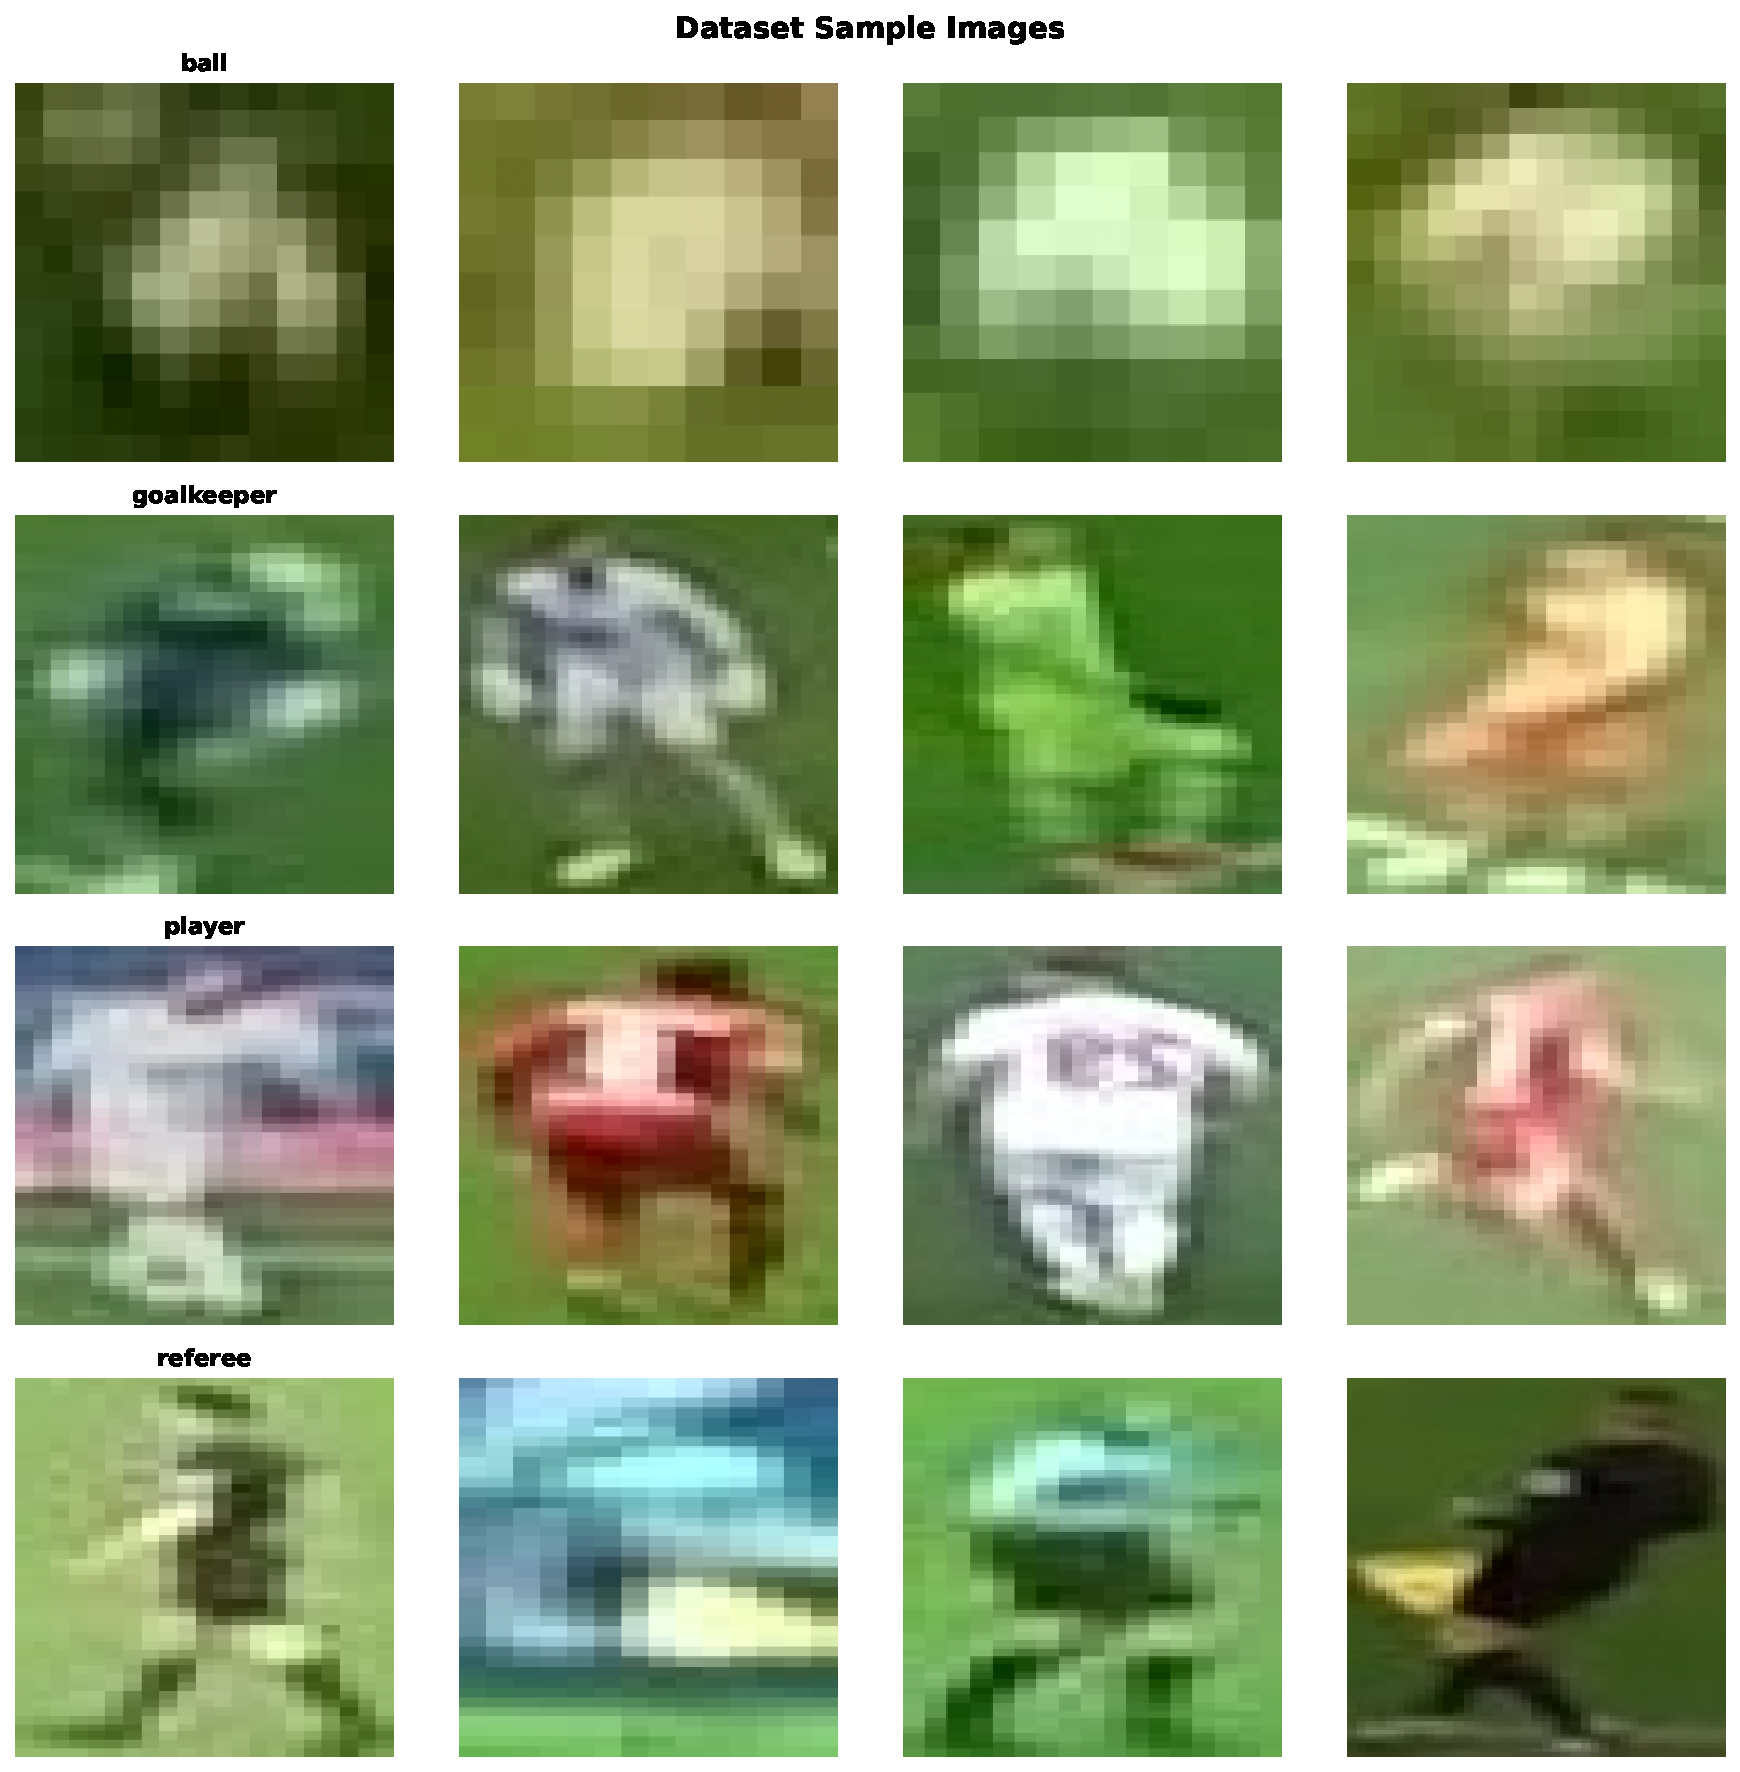
\includegraphics[width=0.95\columnwidth]{sample_images.pdf}
\caption{Representative crops from the dataset, with one row per class showing four examples each of ball, goalkeeper, player, and referee. The figure highlights the strong visual similarity between goalkeepers, outfield players, and referees, which is the principal source of confusion for all models, as well as the very small size of typical ball crops.}
\label{fig:samples}
\end{figure}

\begin{figure}[!ht]
\centering
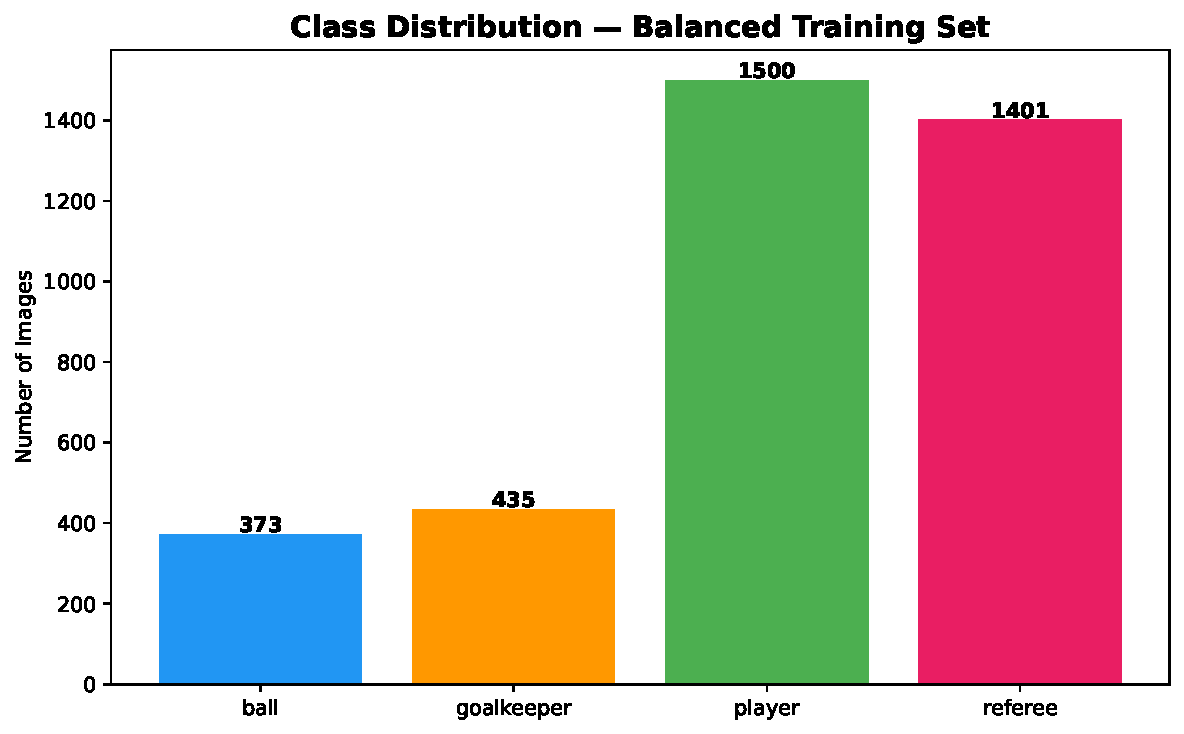
\includegraphics[width=0.8\columnwidth]{class_distribution.pdf}
\caption{Class distribution of the training set after balancing. The minority classes ball and goalkeeper keep all of their available crops, while the majority classes player and referee are capped at 1{,}500 crops through random undersampling applied only to the training split, so that the validation and test partitions retain their natural, imbalanced distribution.}
\label{fig:distribution}
\end{figure}

\subsection{Data Preparation}

\subsubsection{Data Cleaning}
Each annotated bounding box was read from the YOLO label file, converted from normalised to absolute pixel coordinates, and cropped from the source image.
Boxes that produced empty or zero-area regions were skipped, and all valid crops were written to disk organised by split and class.
No label correction was applied because the published annotations were taken as ground truth, and unreadable files were not encountered.

\subsubsection{Data Splitting}
The original match-level partition of 612 training, 38 validation, and 13 test images was preserved, and crops were assigned to the split of their source image.
This produced 15{,}636 crops in total, of which the held-out test split contains 307 crops that remain untouched until the final evaluation.
Preserving the split at the image level guarantees that crops from the same frame never appear in more than one partition, which is the key safeguard against data leakage in this dataset.
No re-splitting or random shuffling across the original partitions was performed.

\subsubsection{Image Preprocessing}
All crops were resized to 224$\times$224 pixels in RGB to match the input dimensions expected by the ImageNet-pretrained backbones~\cite{sandler2018mobilenetv2,he2016deep}.
Pixel intensities were rescaled from the integer range to the floating-point interval $[0,1]$ by dividing by 255.
Resizing uses bilinear interpolation, and no aggressive cropping or contrast manipulation was applied so that the kit-colour cues separating the roles are preserved.
The same preprocessing is applied identically to all three models to keep the comparison fair.

\subsubsection{Data Augmentation}
Label-preserving augmentation is applied on the fly to the training split only, leaving validation and test crops untouched.
The transformations and their ranges are random rotation up to 20 degrees, width and height shifts up to 15\%, zoom up to 15\%, brightness variation between 80\% and 120\%, and horizontal flipping.
Rotation, shifting, and zoom simulate the variability of camera framing and object position, brightness variation reflects changing stadium illumination, and horizontal flipping is valid because role identity is invariant to mirror symmetry.
Extreme colour distortions were deliberately avoided because they could erase the kit-colour information that distinguishes goalkeepers and referees from outfield players, consistent with augmentation guidance in the literature~\cite{lewy2023augmentation}.

\subsubsection{Class-Imbalance Handling}
Two complementary strategies are used to mitigate imbalance.
First, the training split is rebalanced by random undersampling that caps each class at 1{,}500 crops, which reduces the dominance of the player class while retaining every available ball and goalkeeper crop.
Second, class weights inversely proportional to class frequency are passed to the loss so that residual imbalance is penalised during optimisation.
Undersampling is applied only to the training split, and the validation and test splits retain their natural distribution so that the reported metrics reflect realistic deployment conditions~\cite{ghosh2024imbalance}.

\subsection{Model Development}

\subsubsection{Custom CNN Baseline}
The custom CNN takes a 224$\times$224$\times$3 input and stacks four convolutional blocks with 32, 64, 128, and 256 filters respectively.
Each block applies a 3$\times$3 same-padding convolution with ReLU activation, batch normalisation, 2$\times$2 max pooling, and 25\% dropout, so that spatial resolution is progressively reduced while feature depth increases~\cite{ioffe2015batch,srivastava2014dropout}.
The convolutional stack is followed by global average pooling, a 256-unit dense layer with ReLU, batch normalisation, and 50\% dropout, and a final four-unit softmax output.
The network is intentionally compact, with only 458{,}180 trainable parameters, to serve as an efficient from-scratch baseline.
Its structure is summarised in Table~\ref{tab:hyperparams} and the architecture diagram in Figure~\ref{fig:architecture}.

\subsubsection{Transfer-Learning Model One: MobileNetV2}
MobileNetV2, pre-trained on ImageNet, is used as the first transfer-learning backbone with its classification head removed~\cite{sandler2018mobilenetv2,deng2009imagenet}.
A new head is appended consisting of global average pooling, a 512-unit dense layer with ReLU and 40\% dropout, a 256-unit dense layer with ReLU and 30\% dropout, and a four-unit softmax output.
In the first phase the entire backbone is frozen and only the new head is trained, allowing the head to adapt to the four football roles.
In the second phase the last 30 layers of the backbone are unfrozen and trained jointly with the head at a reduced learning rate, fine-tuning high-level features without destroying the pre-trained representation.
The resulting model has roughly 3.05 million parameters.

\subsubsection{Transfer-Learning Model Two: ResNet50}
ResNet50, also pre-trained on ImageNet, is used as the second backbone with the identical custom head described above~\cite{he2016deep}.
The same two-phase strategy is applied, with the last 15 layers unfrozen during fine-tuning, reflecting the deeper structure of the residual network.
This model has approximately 24.8 million parameters, more than fifty times the size of the custom CNN, and serves to test whether additional capacity helps or hurts on this small, imbalanced dataset.

\subsubsection{Feature Extraction and Fine-Tuning Strategy}
Both transfer-learning models follow a two-stage process of frozen-backbone training followed by partial fine-tuning.
Freezing the backbone first stabilises the randomly initialised head and prevents large early gradients from corrupting the pre-trained weights.
Unfreezing only the final layers during fine-tuning concentrates adaptation on the most task-specific features while preserving the generic low-level features, and the number of unfrozen layers (30 for MobileNetV2, 15 for ResNet50) was chosen to balance adaptation against overfitting on limited data.

\subsection{Training Procedure}

\subsubsection{Loss Function}
All models are trained with categorical cross-entropy, the standard loss for mutually exclusive multi-class classification, defined for a single example as
\begin{equation}
\mathcal{L} = -\sum_{c=1}^{C} w_c\, y_c \log(\hat{y}_c),
\label{eq:loss}
\end{equation}
where $C=4$ is the number of roles, $y_c$ is the one-hot ground-truth indicator for class $c$, $\hat{y}_c$ is the predicted probability for class $c$, and $w_c$ is the class weight that compensates for residual imbalance.
The class weights $w_c$ are larger for rarer roles, so that misclassifying a ball or goalkeeper crop incurs a proportionally higher penalty than misclassifying a player crop.

\subsubsection{Optimizer and Learning Rate}
The Adam optimizer is used for all models because of its robust convergence with little manual tuning~\cite{kingma2015adam}.
The initial learning rate is $1\times10^{-3}$ for head training and is reduced for the fine-tuning phase to protect the pre-trained weights.
A ReduceLROnPlateau schedule lowers the learning rate when the validation loss stops improving, and dropout and batch normalisation provide regularisation in place of explicit weight decay.

\subsubsection{Training Controls}
Models are trained with a batch size of 32 for up to 50 epochs per phase, with EarlyStopping monitoring validation accuracy with a patience of 8 epochs.
ModelCheckpoint saves the weights achieving the best validation performance, which are the weights used for all reported results.
A fixed random seed is used where possible for reproducibility, and the best checkpoint rather than the final epoch is always retained.

\subsubsection{Hyperparameter Selection}
Hyperparameter values were chosen from common practice in the transfer-learning literature and lightly adjusted within the constraints of the available single-GPU hardware, rather than through an exhaustive search~\cite{martins2025mobilenet}.
The complete configuration shared across the experiments is reported in Table~\ref{tab:hyperparams}.

\begin{table}[!ht]
\centering
\caption{Training configuration and key architectural settings shared across the three models. Phase~1 trains only the new classification head with the backbone frozen, and phase~2 fine-tunes the final layers of each backbone at a reduced learning rate; the custom CNN is trained in a single phase from random initialisation.}
\label{tab:hyperparams}
\begin{tabular}{ll}
\toprule
\textbf{Setting} & \textbf{Value} \\
\midrule
Input resolution & 224 $\times$ 224 $\times$ 3 \\
Pixel normalisation & rescale to $[0,1]$ \\
Optimizer & Adam \\
Initial learning rate (phase 1) & $1\times10^{-3}$ \\
Fine-tuning learning rate (phase 2) & $1\times10^{-5}$ \\
Loss & weighted categorical cross-entropy \\
Batch size & 32 \\
Maximum epochs per phase & 50 \\
Early stopping patience & 8 epochs (val.\ accuracy) \\
LR schedule & ReduceLROnPlateau (val.\ loss) \\
Dropout (conv blocks / dense) & 0.25 / 0.5 \\
Unfrozen layers (MobileNetV2 / ResNet50) & 30 / 15 \\
Balancing cap per class (train only) & 1{,}500 crops \\
Class weights & inverse class frequency \\
Custom CNN parameters & 458{,}180 \\
MobileNetV2 parameters & 3{,}046{,}212 \\
ResNet50 parameters & 24{,}769{,}156 \\
\bottomrule
\end{tabular}
\end{table}

% TODO (author): draw the custom-CNN architecture (four conv blocks -> GAP ->
% dense -> softmax) in PowerPoint/Visio and save as Figures/architecture.pdf.
\begin{figure*}[!ht]
\centerline{\includegraphics[width=15cm]{Figures/architecture.pdf}}
\caption{Architecture of the custom CNN baseline. The 224$\times$224$\times$3 input passes through four convolutional blocks with 32, 64, 128, and 256 filters, each combining a 3$\times$3 convolution, batch normalisation, 2$\times$2 max pooling, and dropout, followed by global average pooling, a 256-unit dense layer with dropout, and a four-unit softmax output producing the ball, goalkeeper, player, and referee probabilities.}
\label{fig:architecture}
\end{figure*}

\subsection{Evaluation Framework}

\subsubsection{Primary Predictive Metrics}
Predictive performance is reported with accuracy, precision, recall, and F1-score, all defined with respect to the four football roles rather than as abstract ratios.
For a given role $c$, a true positive is a crop of role $c$ correctly predicted as $c$, a false positive is a crop of another role predicted as $c$, and a false negative is a crop of role $c$ predicted as another role.
Accuracy is the fraction of all test crops whose predicted role matches the annotated role,
\begin{equation}
\text{Accuracy} = \frac{\text{correctly classified crops}}{\text{total crops}}.
\label{eq:acc}
\end{equation}
Per-class precision and recall are
\begin{equation}
\text{Precision}_c = \frac{TP_c}{TP_c + FP_c}, \qquad
\text{Recall}_c = \frac{TP_c}{TP_c + FN_c},
\label{eq:pr}
\end{equation}
so that precision for the goalkeeper class measures how many crops predicted as goalkeeper truly are goalkeepers, and recall measures how many actual goalkeepers were found.
The per-class F1-score is the harmonic mean of precision and recall, and the macro F1-score averages it equally over the four roles,
\begin{equation}
\text{F1}_c = \frac{2\,\text{Precision}_c\,\text{Recall}_c}{\text{Precision}_c + \text{Recall}_c}, \qquad
\text{macro F1} = \frac{1}{C}\sum_{c=1}^{C}\text{F1}_c.
\label{eq:f1}
\end{equation}
The macro F1-score is the primary selection metric because it weights every role equally and therefore exposes failures on the rare ball and goalkeeper classes that accuracy would hide.

\subsubsection{Class-Level Evaluation}
For every model the full confusion matrix is computed on both the validation and the held-out test split, together with the per-class precision, recall, and F1-score.
Particular attention is paid to minority-class behaviour, because the dataset is dominated by the player class and a model that ignores the rare classes can still score highly on accuracy.

\subsubsection{Training Behaviour}
Training and validation accuracy and loss curves are recorded for each model to assess convergence, overfitting, and stability.
The epoch of best validation performance and the early-stopping point are noted, and divergence between training and validation curves is used to diagnose overfitting.

\subsubsection{Computational Efficiency}
Efficiency is reported through the trainable parameter count and the on-disk model size in megabytes for each model.
These quantities directly affect memory footprint and suitability for deployment on modest hardware, which is central to the low-resource motivation of the study.

\subsubsection{Statistical Reliability}
Because training each model is computationally expensive on a single GPU, results are reported from the best-checkpoint model of a single run rather than from repeated runs.
Differences that fall within the noise of a single run are therefore discussed qualitatively, and no claim of statistical significance is made for small accuracy gaps; repeated runs with confidence intervals are identified as future work.

\subsection{Explainable AI Methodology}

\subsubsection{Grad-CAM Procedure}
Grad-CAM heatmaps are generated from the last convolutional layer of each model with respect to the predicted class~\cite{selvaraju2020gradcam}.
The class-score gradients are global-average-pooled to obtain channel importance weights, combined with the forward activations, passed through a ReLU, normalised to $[0,1]$, and upsampled and overlaid on the original crop.
Example crops are selected to cover correct and incorrect predictions across all four roles so that the attention patterns can be compared between successes and failures.

\subsubsection{SHAP Procedure}
SHAP explanations are produced with a model-agnostic Partition explainer using an inpainting image masker, which relies only on the model's forward pass and is therefore robust across framework versions~\cite{lundberg2017unified}.
Two test crops per class are explained, and for each crop the attribution map for the predicted class is computed with 600 masking evaluations, yielding regions of positive (supporting) and negative (opposing) evidence.
Positive regions are interpreted as image areas that increase the predicted-class probability, and negative regions as areas that decrease it.

\subsubsection{Explanation Assessment}
Explanations are judged by whether attention and attribution fall on the target object, such as the player's torso or the ball, rather than on background pitch or crowd.
Agreement between Grad-CAM and SHAP is treated as stronger evidence of meaningful reasoning, and systematic differences between correct and incorrect predictions are highlighted.
A model whose explanations consistently ignore the object while still scoring highly is flagged as relying on a shortcut, consistent with the cautions raised in the explainability literature~\cite{nazir2023survey}.

\subsection{Robustness Analysis}
Robustness is evaluated by corrupting the held-out test crops with five degradations representative of broadcast conditions, namely Gaussian blur, additive Gaussian noise, reduced brightness, central occlusion, and JPEG compression, each at five severity levels with level zero denoting the clean image~\cite{hendrycks2019benchmarking}.
For every corruption and severity the entire test set is transformed and re-classified, and accuracy and macro F1-score are recorded per model.
This protocol reveals not only how quickly each model degrades but also whether a model is pathologically invariant to corruption, which would indicate that it ignores the image content.

\subsection{Software, Hardware, and Reproducibility}
All experiments were implemented in Python with TensorFlow and Keras~\cite{tensorflow2015} and run on a workstation equipped with an NVIDIA GeForce RTX 3080 GPU.
SHAP was used for the attribution analysis, OpenCV and NumPy for image corruption, and scikit-learn for the classification metrics.
The pipeline is organised into separate scripts for dataset preparation, balancing, training, Grad-CAM, SHAP, robustness, and inference, and the trained models and all generated figures are saved to a dedicated outputs directory.
A reproducible Kaggle notebook accompanies the project, and the source code is intended to be released in a public repository so that the full experiment can be reproduced.

\subsection{Ethical and Practical Considerations}
The dataset contains images of people in a public sporting context and is used under its CC BY 4.0 licence, but broadcast footage can still raise privacy and consent concerns if extended to identification rather than role classification.
The strong class imbalance means that minority roles are represented by few examples, so any downstream use must account for unequal reliability across roles.
Because the system can fail on visually similar roles, its outputs should support rather than replace human judgement, particularly if ever connected to officiating, and high-stakes decisions require human oversight.
The framework is therefore positioned as a decision-support tool, not an autonomous arbiter.

\section{Results}
\label{sec:results}

\subsection{Dataset and Preprocessing Results}
Crop extraction from the 663 annotated match images produced 15{,}636 usable object crops, with no files discarded as corrupt or unreadable.
The raw class distribution is extremely skewed, with outfield players accounting for more than thirteen thousand crops and the ball for only a few hundred, confirming the imbalance anticipated in the dataset description.
After training-only balancing the player and referee classes were capped at 1{,}500 crops while ball and goalkeeper retained all available crops, substantially reducing the dominance of the player class in the training set as shown in Figure~\ref{fig:distribution}.
The match-level split was preserved exactly, yielding a held-out test partition of 307 crops whose natural, imbalanced distribution is retained, with players forming 258 of the 307 test crops.
Representative crops in Figure~\ref{fig:samples} confirm the strong visual similarity between goalkeepers, referees, and outfield players and the very small size of typical ball crops.
These observations directly motivate RQ1 and RQ3, because the imbalance and inter-class similarity define the difficulty of the task.

\subsection{Training and Convergence Results}
Figures~\ref{fig:curves_cnn},~\ref{fig:curves_mobile}, and~\ref{fig:curves_resnet} show the training and validation accuracy and loss curves for the three models.
The custom CNN converges smoothly and its validation accuracy tracks its training accuracy without a large gap, indicating limited overfitting for a model of its size.
MobileNetV2 converges quickly during head training and improves further during fine-tuning, with some fluctuation in the validation curve.
ResNet50 reaches a high validation accuracy almost immediately and then plateaus, a pattern that the later class-level analysis shows to be the signature of collapse onto the majority class rather than genuine learning of all roles.
Early stopping halted each run once validation accuracy stopped improving, and the best-checkpoint weights were retained for evaluation.

\begin{figure}[!ht]
\centering
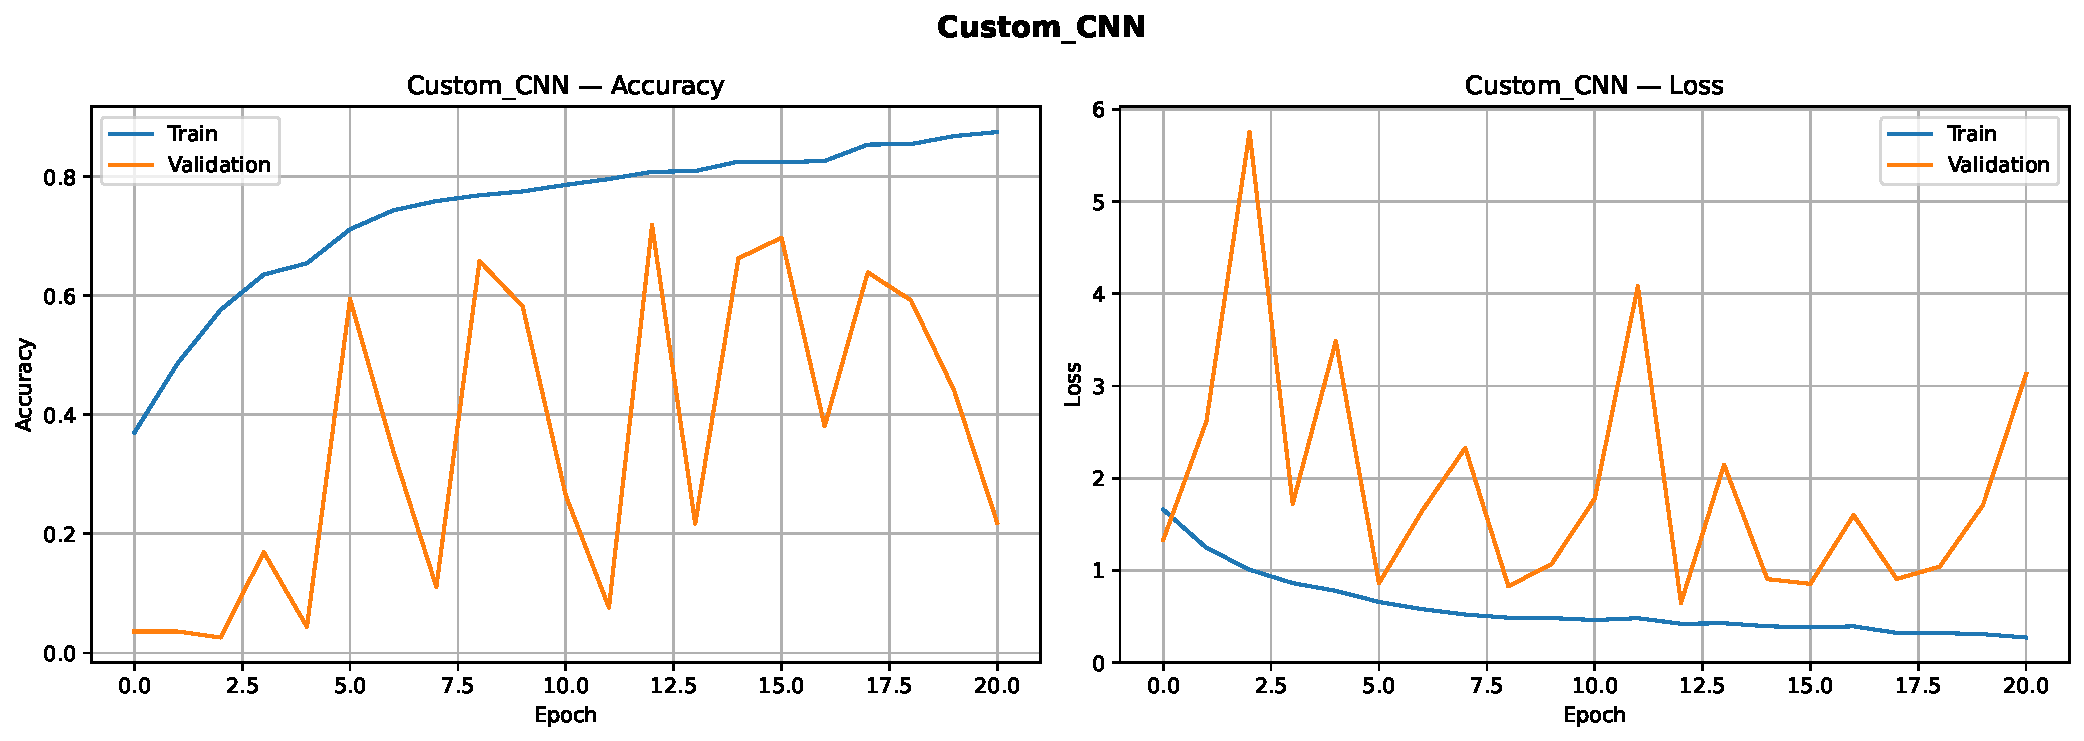
\includegraphics[width=0.95\columnwidth]{curves_Custom_CNN.pdf}
\caption{Training and validation accuracy and loss curves for the custom CNN. The validation curve closely follows the training curve, indicating stable convergence and limited overfitting for the 0.46M-parameter baseline.}
\label{fig:curves_cnn}
\end{figure}

\begin{figure}[!ht]
\centering
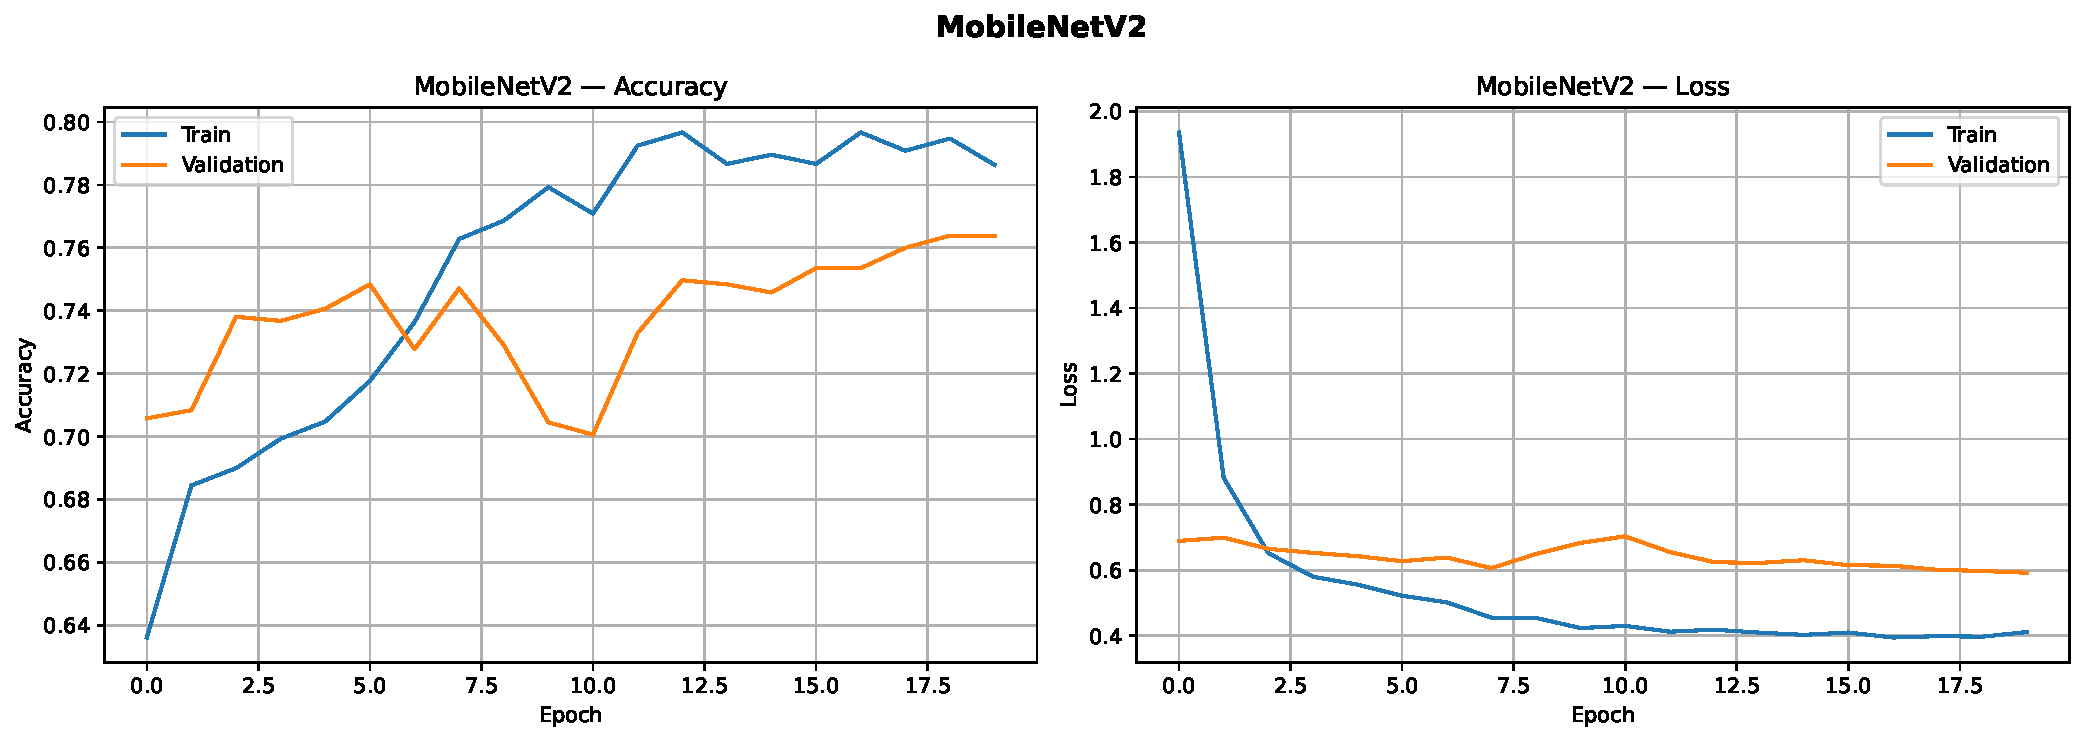
\includegraphics[width=0.95\columnwidth]{curves_MobileNetV2.pdf}
\caption{Training and validation accuracy and loss curves for MobileNetV2 during the fine-tuning phase. The model converges rapidly after the backbone is partially unfrozen, with moderate fluctuation in the validation accuracy.}
\label{fig:curves_mobile}
\end{figure}

\begin{figure}[!ht]
\centering
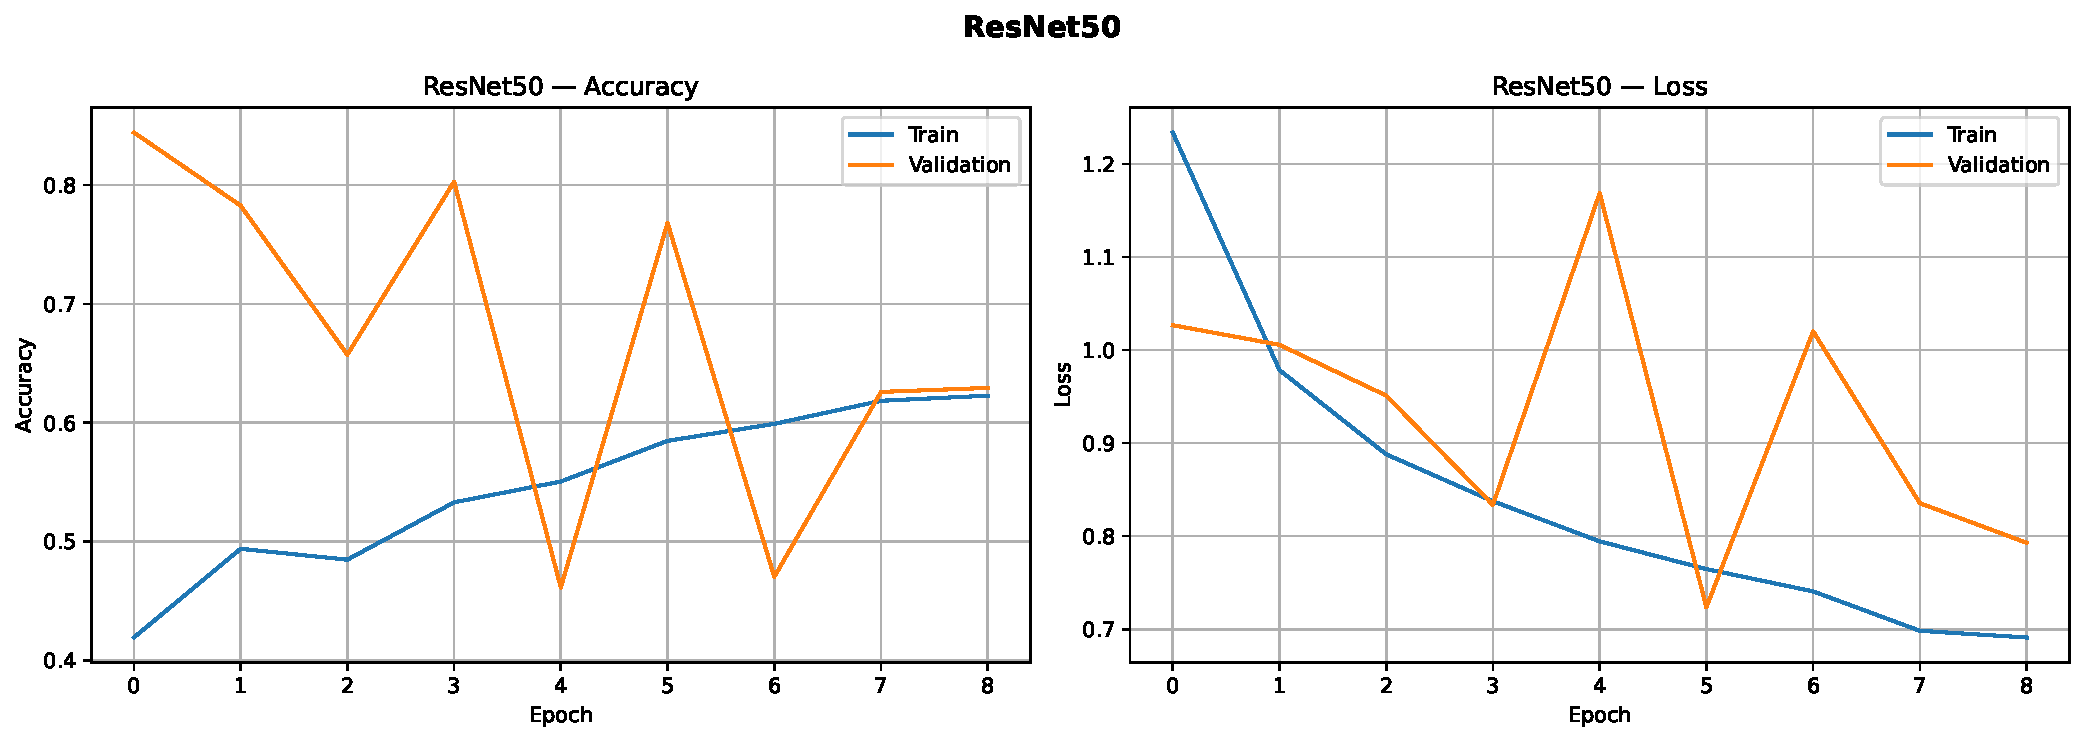
\includegraphics[width=0.95\columnwidth]{curves_ResNet50.pdf}
\caption{Training and validation accuracy and loss curves for ResNet50 during the fine-tuning phase. Validation accuracy saturates almost immediately near the majority-class proportion, foreshadowing the degenerate behaviour revealed by the per-class analysis.}
\label{fig:curves_resnet}
\end{figure}

\subsection{Overall Model Performance}
Table~\ref{tab:results} reports the main comparison on the held-out test split, including accuracy, macro precision, recall, and F1-score, weighted F1-score, parameter count, and model size.
ResNet50 attains the highest raw test accuracy at 84.0\%, but its macro F1-score is only 0.23, far below the other two models.
The custom CNN achieves 77.9\% accuracy with a macro F1-score of 0.67, the best balanced performance of the three, while MobileNetV2 reaches 69.1\% accuracy and a macro F1-score of 0.60.
The same ordering holds on the validation split, where accuracies are 71.9\%, 67.1\%, and 84.4\% for the custom CNN, MobileNetV2, and ResNet50 respectively.
Crucially, the model with the highest accuracy is the worst by macro F1-score, which means that the numerically strongest model by the headline metric is the weakest once every role is weighted equally.
The accuracy comparison is visualised in Figure~\ref{fig:comparison}.
These results address RQ2, and they show that accuracy and macro F1-score point to opposite conclusions on this imbalanced task.

\begin{table}[!ht]
\centering
\caption{Performance of the three models on the held-out test split of 307 crops. Macro metrics weight all four roles equally, whereas the weighted F1-score is dominated by the majority player class. ResNet50 attains the highest accuracy but the lowest macro F1-score, because it predicts ``player'' for every crop; the compact custom CNN gives the best balanced performance.}
\label{tab:results}
\begin{tabular}{lccccccc}
\toprule
\textbf{Model} & \textbf{Acc.} & \textbf{Macro P} & \textbf{Macro R} & \textbf{Macro F1} & \textbf{Weighted F1} & \textbf{Params} & \textbf{Size} \\
\midrule
Custom CNN & \textbf{77.9\%} & \textbf{0.70} & \textbf{0.80} & \textbf{0.67} & \textbf{0.82} & 0.46M & 5.4\,MB \\
MobileNetV2 & 69.1\% & 0.59 & 0.74 & 0.60 & 0.76 & 3.05M & 30\,MB \\
ResNet50 & 84.0\% & 0.21 & 0.25 & 0.23 & 0.77 & 24.8M & 147\,MB \\
\bottomrule
\end{tabular}
\end{table}

\begin{figure}[!ht]
\centering
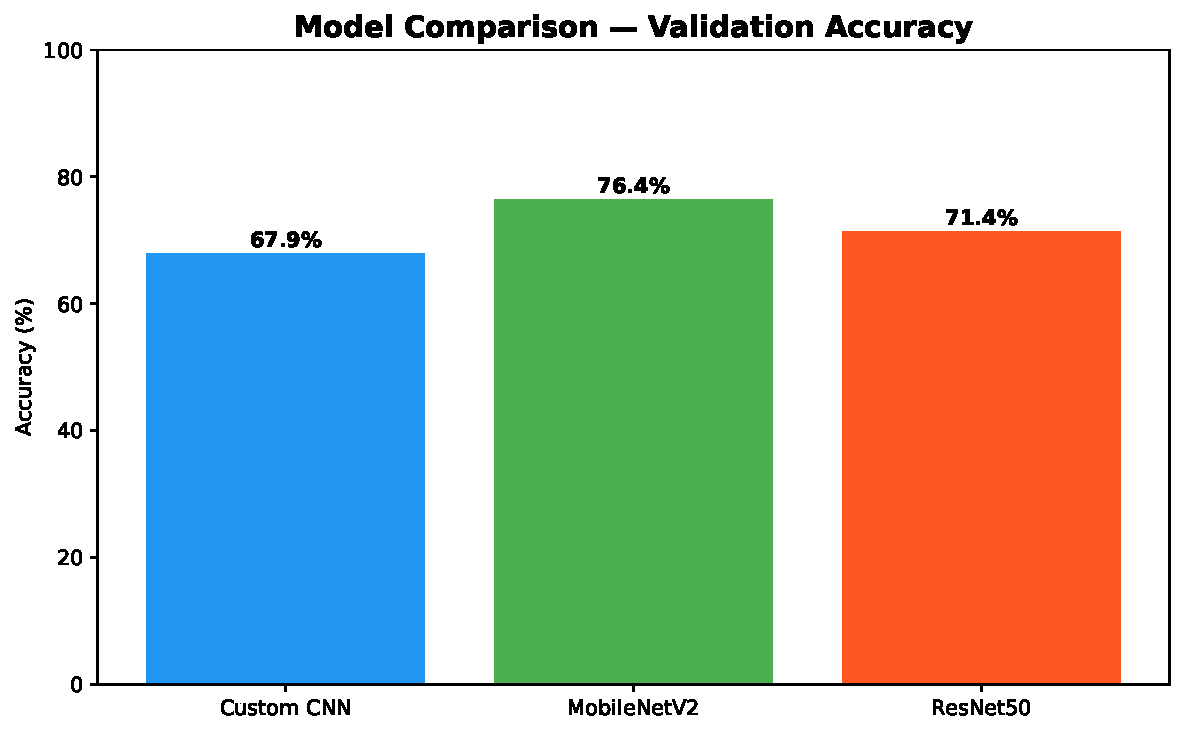
\includegraphics[width=0.85\columnwidth]{model_comparison.pdf}
\caption{Test-set accuracy comparison across the three models. ResNet50 reports the highest accuracy, but this figure must be read together with Table~\ref{tab:results}, because the same model has by far the lowest macro F1-score owing to its collapse onto the majority class.}
\label{fig:comparison}
\end{figure}

\subsection{Class-Level Performance}
The per-class test results in Table~\ref{tab:perclass} explain the divergence between accuracy and macro F1-score.
The custom CNN classifies the ball almost perfectly (F1 0.94) and the player class well (F1 0.87), while struggling most with the goalkeeper class (F1 0.30) and achieving moderate referee performance (F1 0.58).
MobileNetV2 shows a similar profile with strong ball (F1 0.82) and player (F1 0.80) performance and weak goalkeeper performance (F1 0.18).
ResNet50, by contrast, obtains an F1-score of exactly 0.00 for ball, goalkeeper, and referee, and 0.91 for player, because it predicts ``player'' for every single test crop.
This degenerate behaviour is what allows ResNet50 to post 84.0\% accuracy, since players make up 84\% of the test crops, while completely failing on the three minority roles.
The corresponding test confusion matrices in Figures~\ref{fig:cm_cnn},~\ref{fig:cm_mobile}, and~\ref{fig:cm_resnet} make this visually explicit, with ResNet50 placing all mass in the player column.
These findings directly address RQ3, confirming that the goalkeeper class is the hardest for the discriminative models and that the deepest model fails on every minority class.

\begin{table}[!ht]
\centering
\caption{Per-class F1-score on the held-out test split for the three models, with the number of test crops per class in parentheses. ResNet50 scores zero on the three minority roles because it never predicts anything other than ``player''.}
\label{tab:perclass}
\begin{tabular}{lcccc}
\toprule
\textbf{Model} & \textbf{Ball (9)} & \textbf{Goalkeeper (11)} & \textbf{Player (258)} & \textbf{Referee (29)} \\
\midrule
Custom CNN & \textbf{0.94} & \textbf{0.30} & 0.87 & \textbf{0.58} \\
MobileNetV2 & 0.82 & 0.18 & 0.80 & 0.59 \\
ResNet50 & 0.00 & 0.00 & \textbf{0.91} & 0.00 \\
\bottomrule
\end{tabular}
\end{table}

\begin{figure}[!ht]
\centering
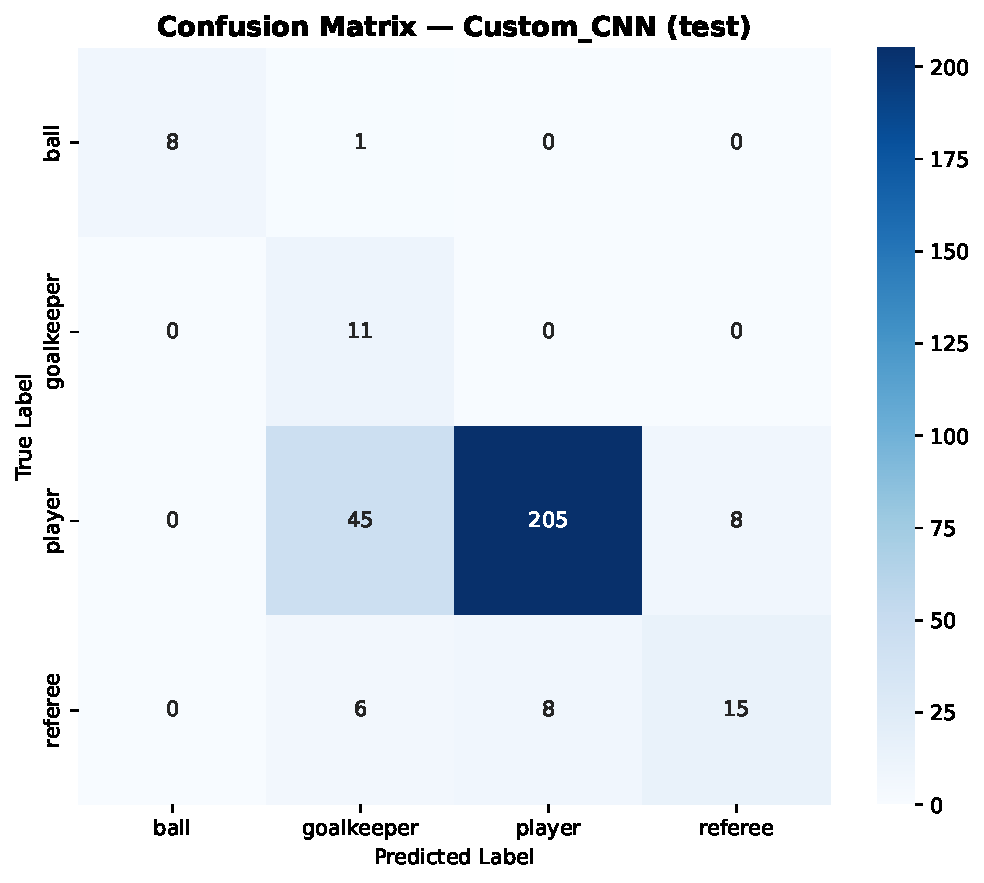
\includegraphics[width=0.7\columnwidth]{cm_Custom_CNN_test.pdf}
\caption{Test-set confusion matrix for the custom CNN. Most errors involve confusing goalkeepers and referees with outfield players, which is expected given their visual similarity, but every role receives a substantial number of correct predictions.}
\label{fig:cm_cnn}
\end{figure}

\begin{figure}[!ht]
\centering
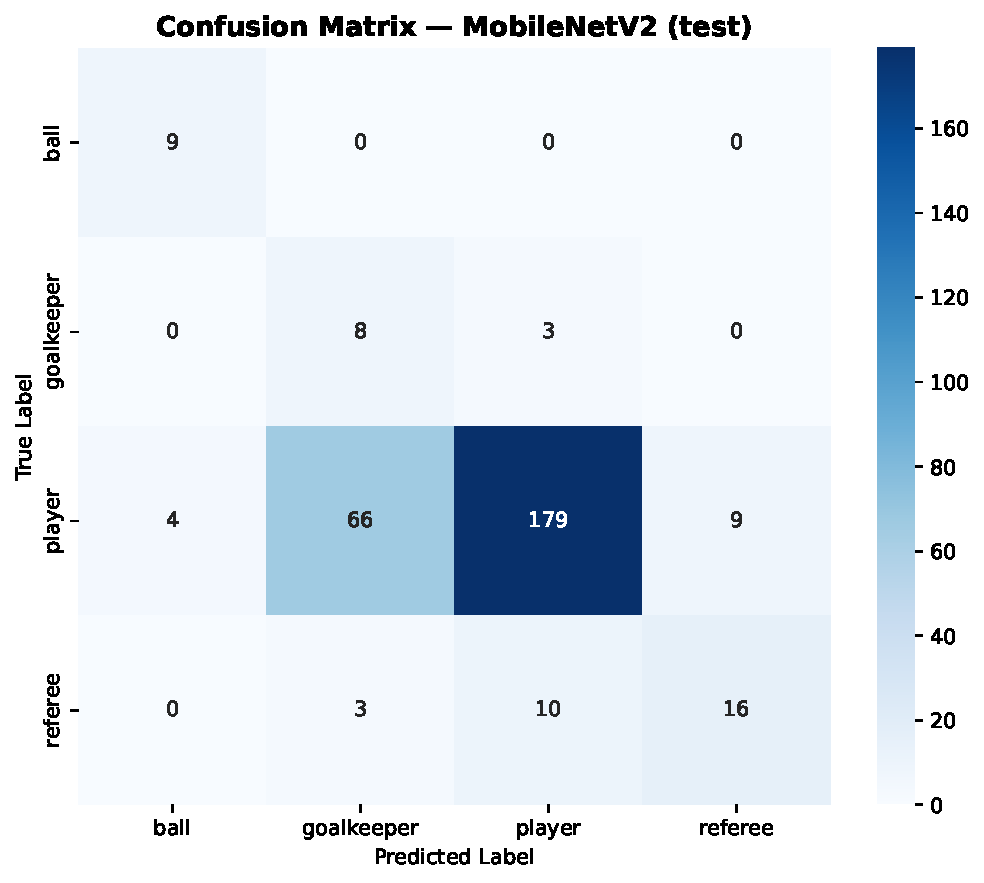
\includegraphics[width=0.7\columnwidth]{cm_MobileNetV2_test.pdf}
\caption{Test-set confusion matrix for MobileNetV2. The pattern resembles that of the custom CNN, with the goalkeeper class being the most frequently confused, but with slightly lower overall balance.}
\label{fig:cm_mobile}
\end{figure}

\begin{figure}[!ht]
\centering
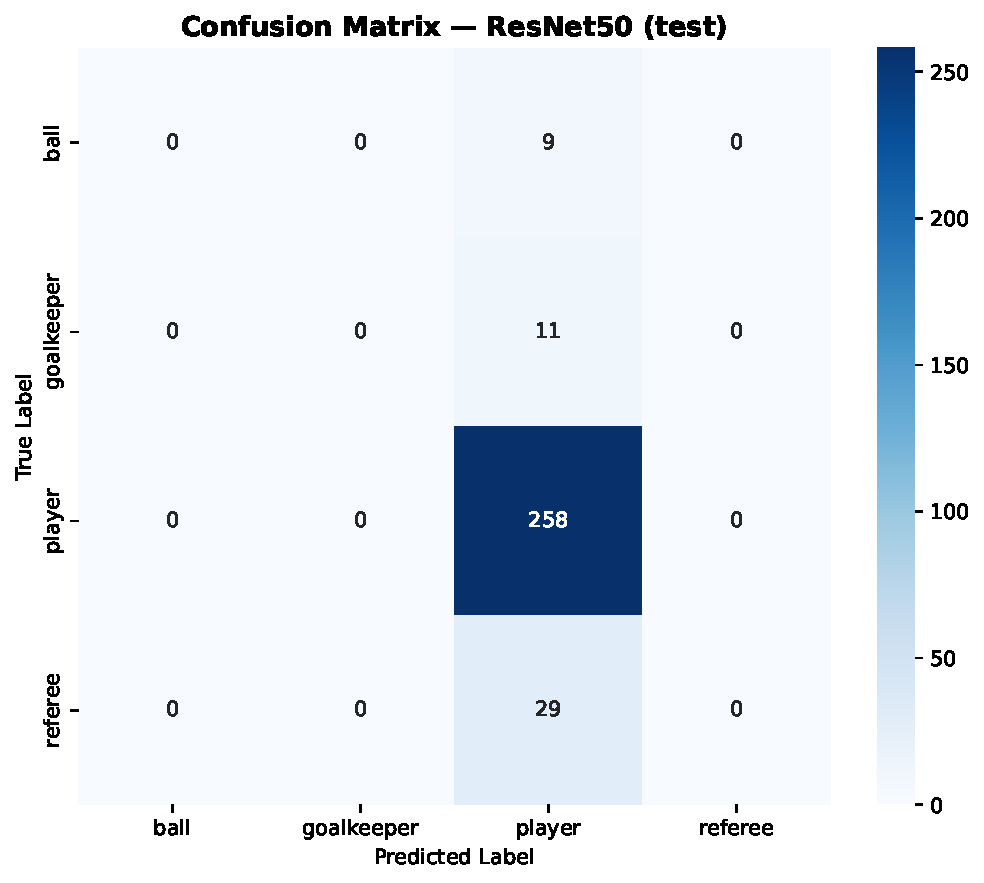
\includegraphics[width=0.7\columnwidth]{cm_ResNet50_test.pdf}
\caption{Test-set confusion matrix for ResNet50. The entire probability mass falls in the player column, visually confirming that the model has collapsed onto the majority class and ignores the ball, goalkeeper, and referee roles entirely.}
\label{fig:cm_resnet}
\end{figure}

\subsection{Explainable AI Results}

\subsubsection{Grad-CAM Results}
Figures~\ref{fig:gradcam_cnn},~\ref{fig:gradcam_mobile}, and~\ref{fig:gradcam_resnet} show Grad-CAM heatmaps for representative crops from each model, with correct predictions marked in green and incorrect ones in red.
For the custom CNN the attention concentrates on the body of the player and the round region of the ball, which is the expected evidence for these roles.
MobileNetV2 produces similarly focused heatmaps on the object of interest for its correct predictions, especially for the ball and player classes.
ResNet50 produces heatmaps that are diffuse and only loosely tied to the object, consistent with a model that is not using class-specific evidence.

\subsubsection{SHAP Results}
Figures~\ref{fig:shap_cnn},~\ref{fig:shap_mobile}, and~\ref{fig:shap_resnet} show SHAP attribution maps for two test crops per class, with positive (supporting) and negative (opposing) regions for the predicted class.
For the custom CNN and MobileNetV2 the positive attributions fall predominantly on the object itself, such as the torso of the player or the body of the ball, indicating that the prediction is driven by relevant pixels.
For ResNet50 the attributions are weak and scattered across the background, reflecting that the prediction is essentially independent of the specific image content because the model always outputs the player class.

\subsubsection{Explanation Comparison}
Grad-CAM and SHAP largely agree for the custom CNN and MobileNetV2, both highlighting the object of interest, which strengthens confidence that these models reason from meaningful regions.
For ResNet50 both methods agree in the opposite sense, neither showing consistent object-focused evidence, which independently corroborates the degenerate behaviour seen in the confusion matrix.
This convergence between two different explanation methods, and between the explanations and the quantitative metrics, addresses RQ4 by showing that the high-accuracy model is not trustworthy.

\begin{figure}[!ht]
\centering
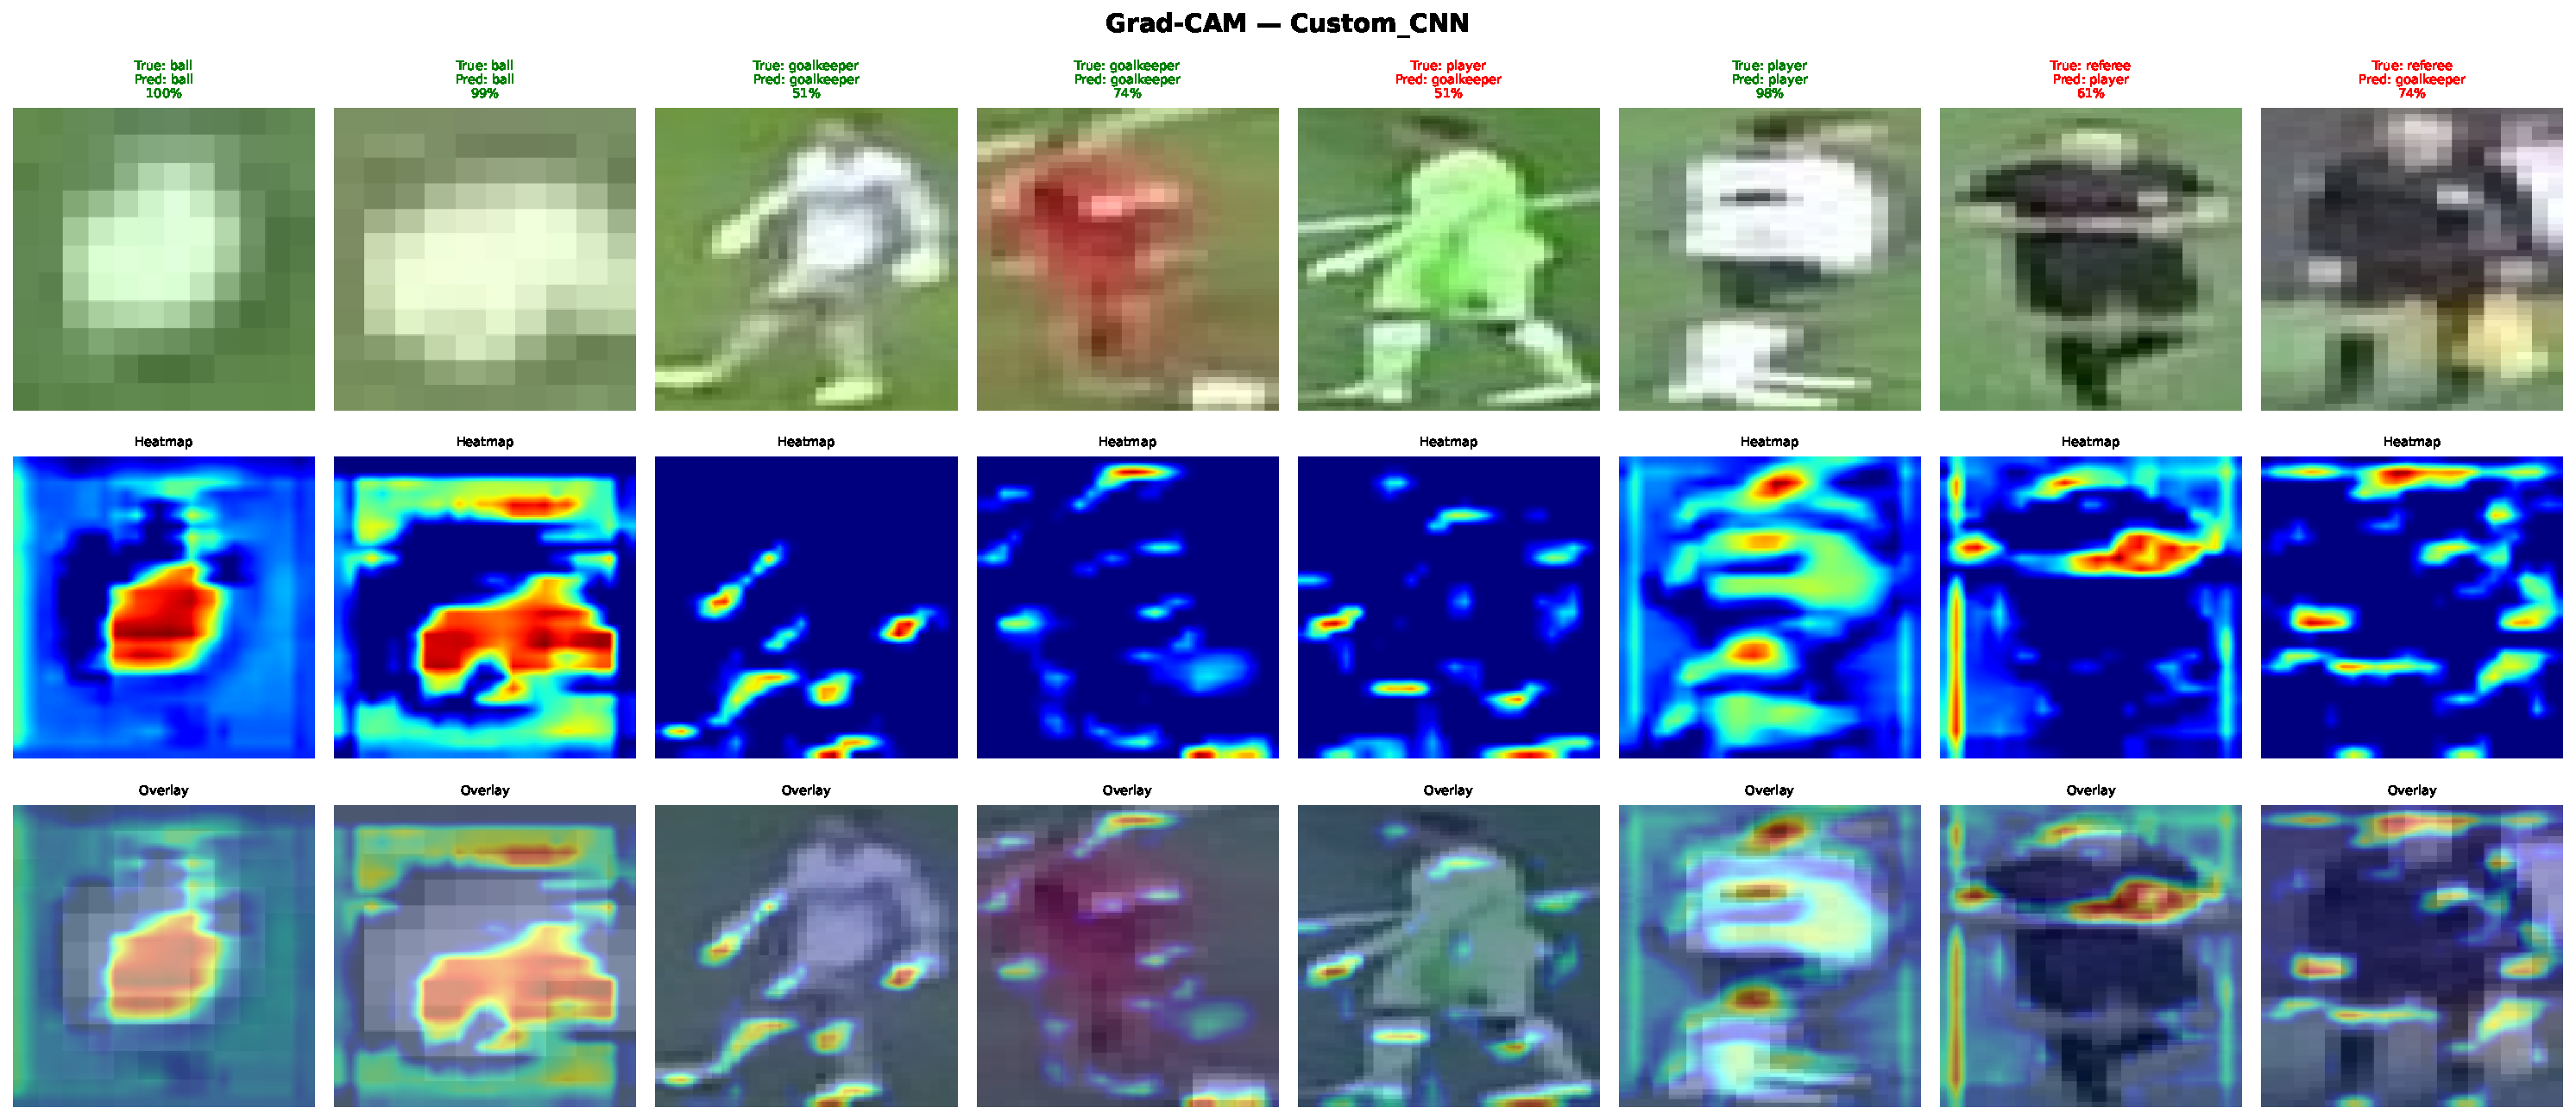
\includegraphics[width=0.95\columnwidth]{gradcam_Custom_CNN.pdf}
\caption{Grad-CAM visualisations for the custom CNN. Green titles denote correct predictions and red titles denote errors; attention concentrates on the player body and the ball, indicating object-focused reasoning.}
\label{fig:gradcam_cnn}
\end{figure}

\begin{figure}[!ht]
\centering
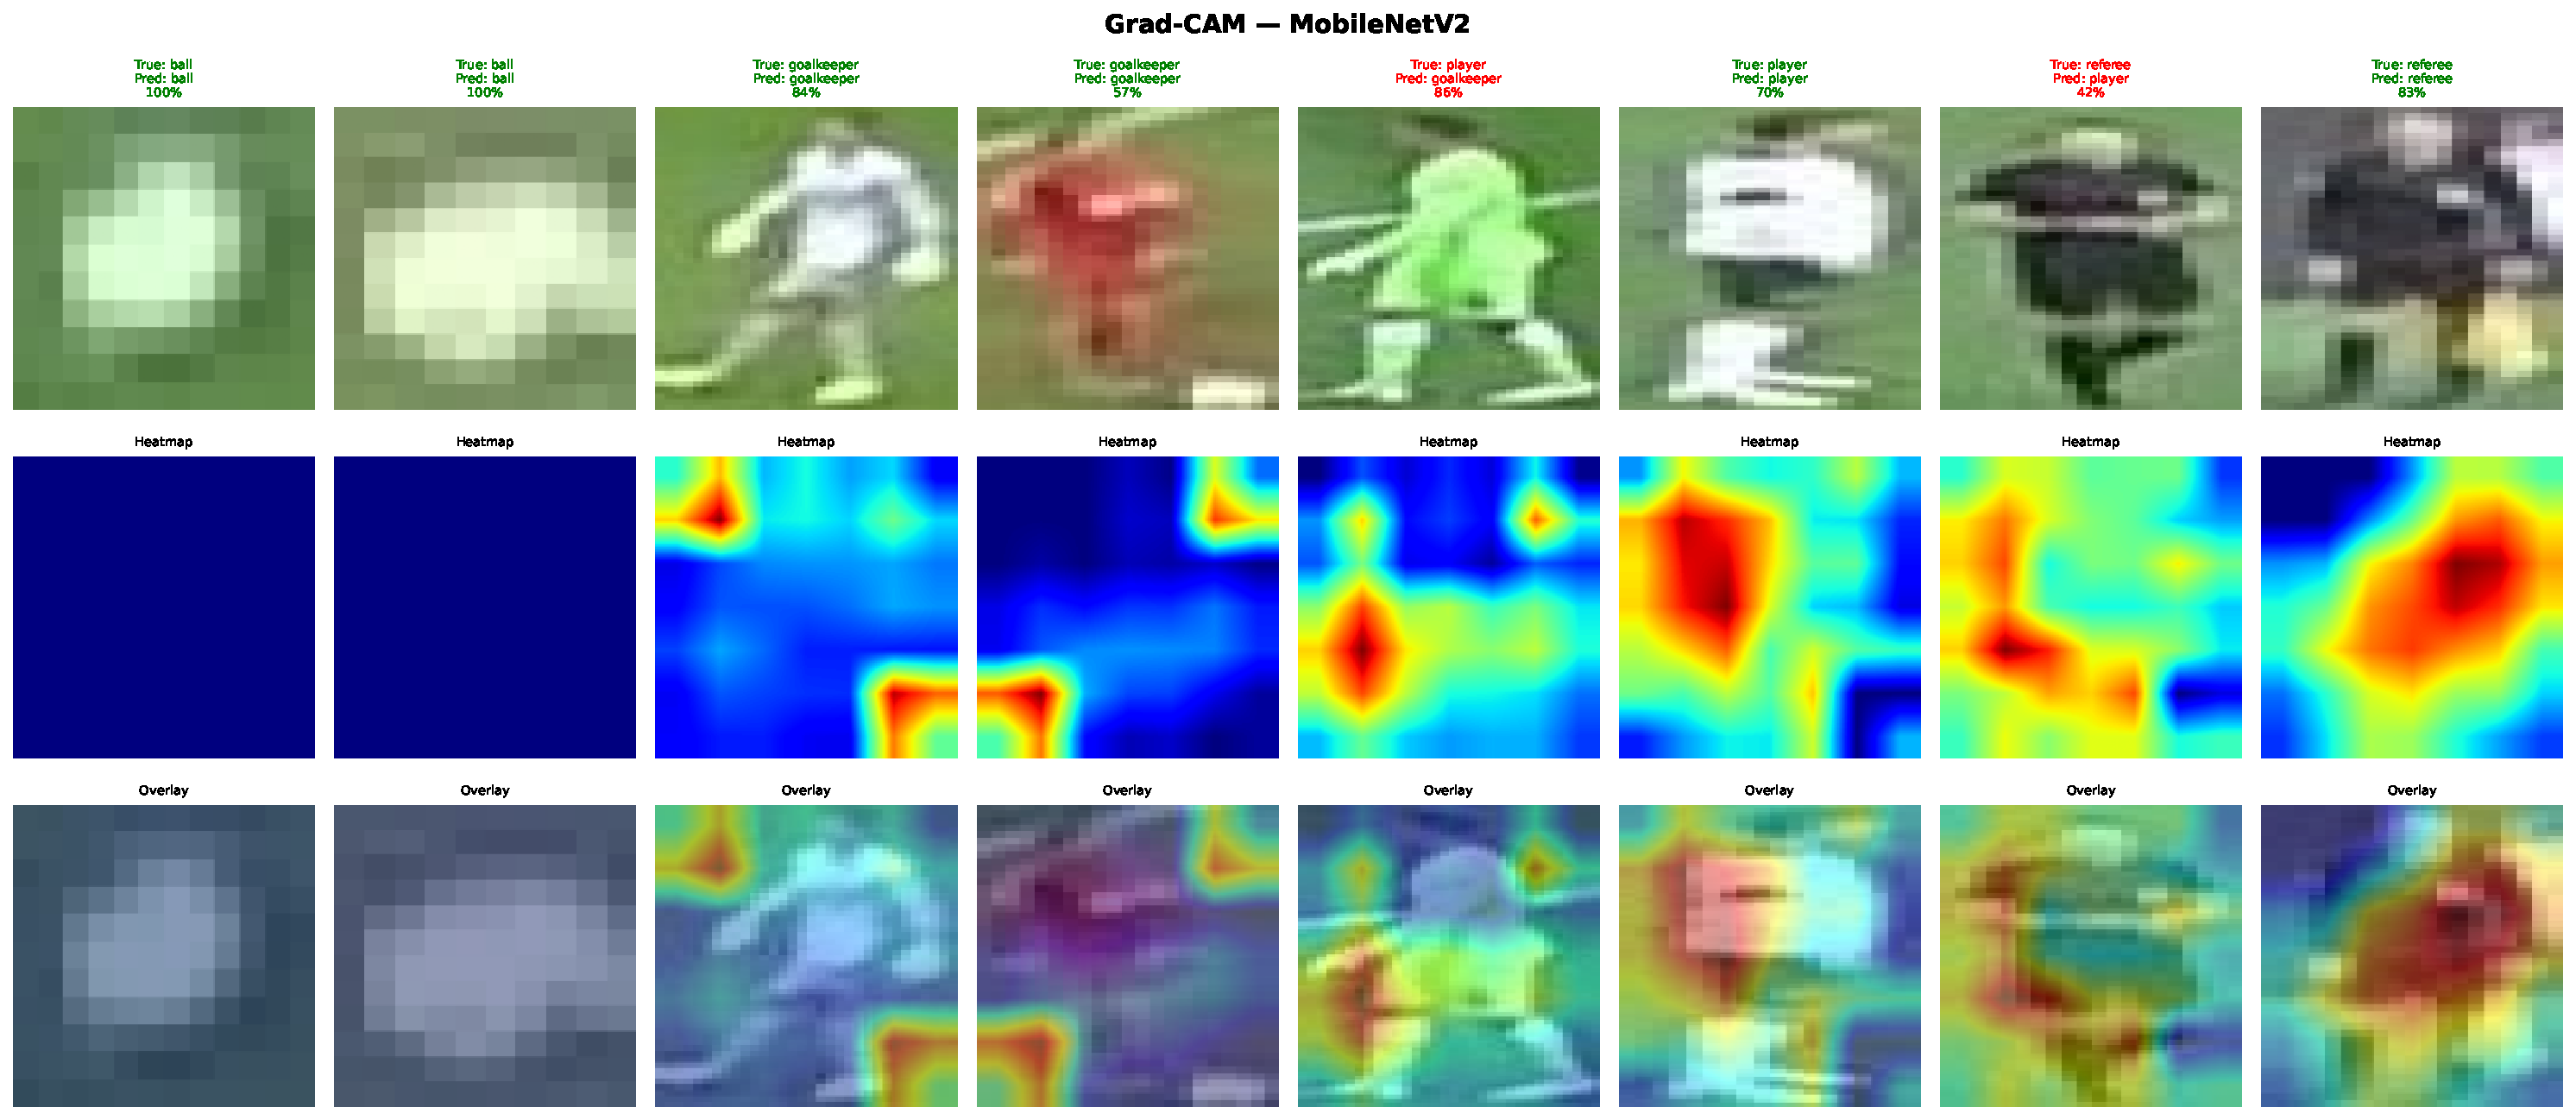
\includegraphics[width=0.95\columnwidth]{gradcam_MobileNetV2.pdf}
\caption{Grad-CAM visualisations for MobileNetV2. The heatmaps remain focused on the object of interest for correct predictions, particularly for the ball and player classes.}
\label{fig:gradcam_mobile}
\end{figure}

\begin{figure}[!ht]
\centering
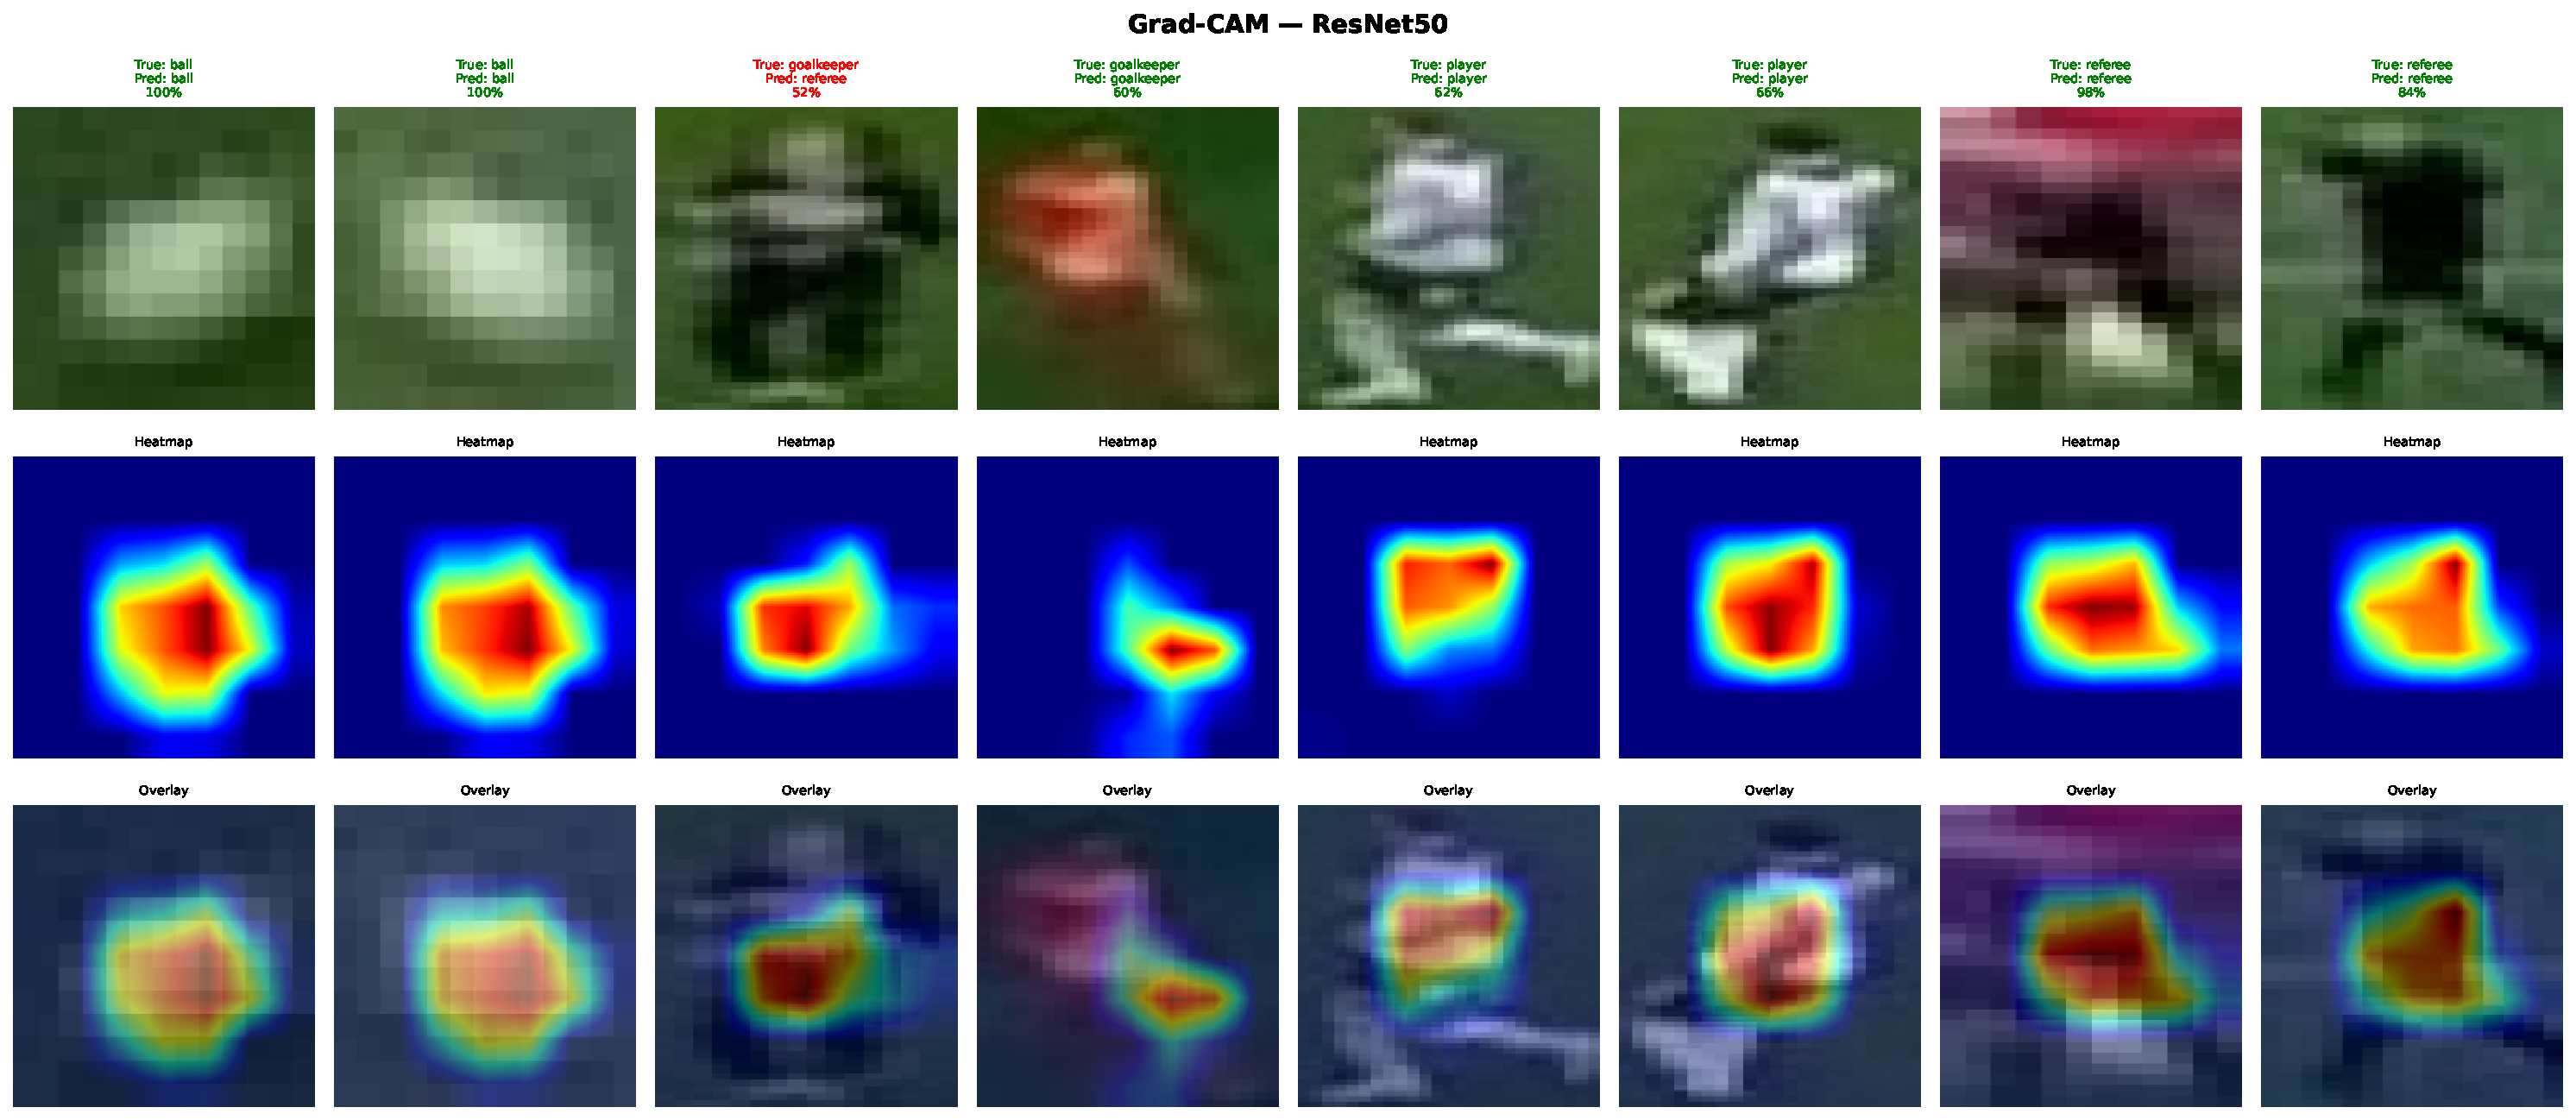
\includegraphics[width=0.95\columnwidth]{gradcam_ResNet50.pdf}
\caption{Grad-CAM visualisations for ResNet50. The heatmaps are diffuse and weakly tied to the object, consistent with a model that does not use class-specific evidence and predicts the majority class regardless of input.}
\label{fig:gradcam_resnet}
\end{figure}

\begin{figure}[!ht]
\centering
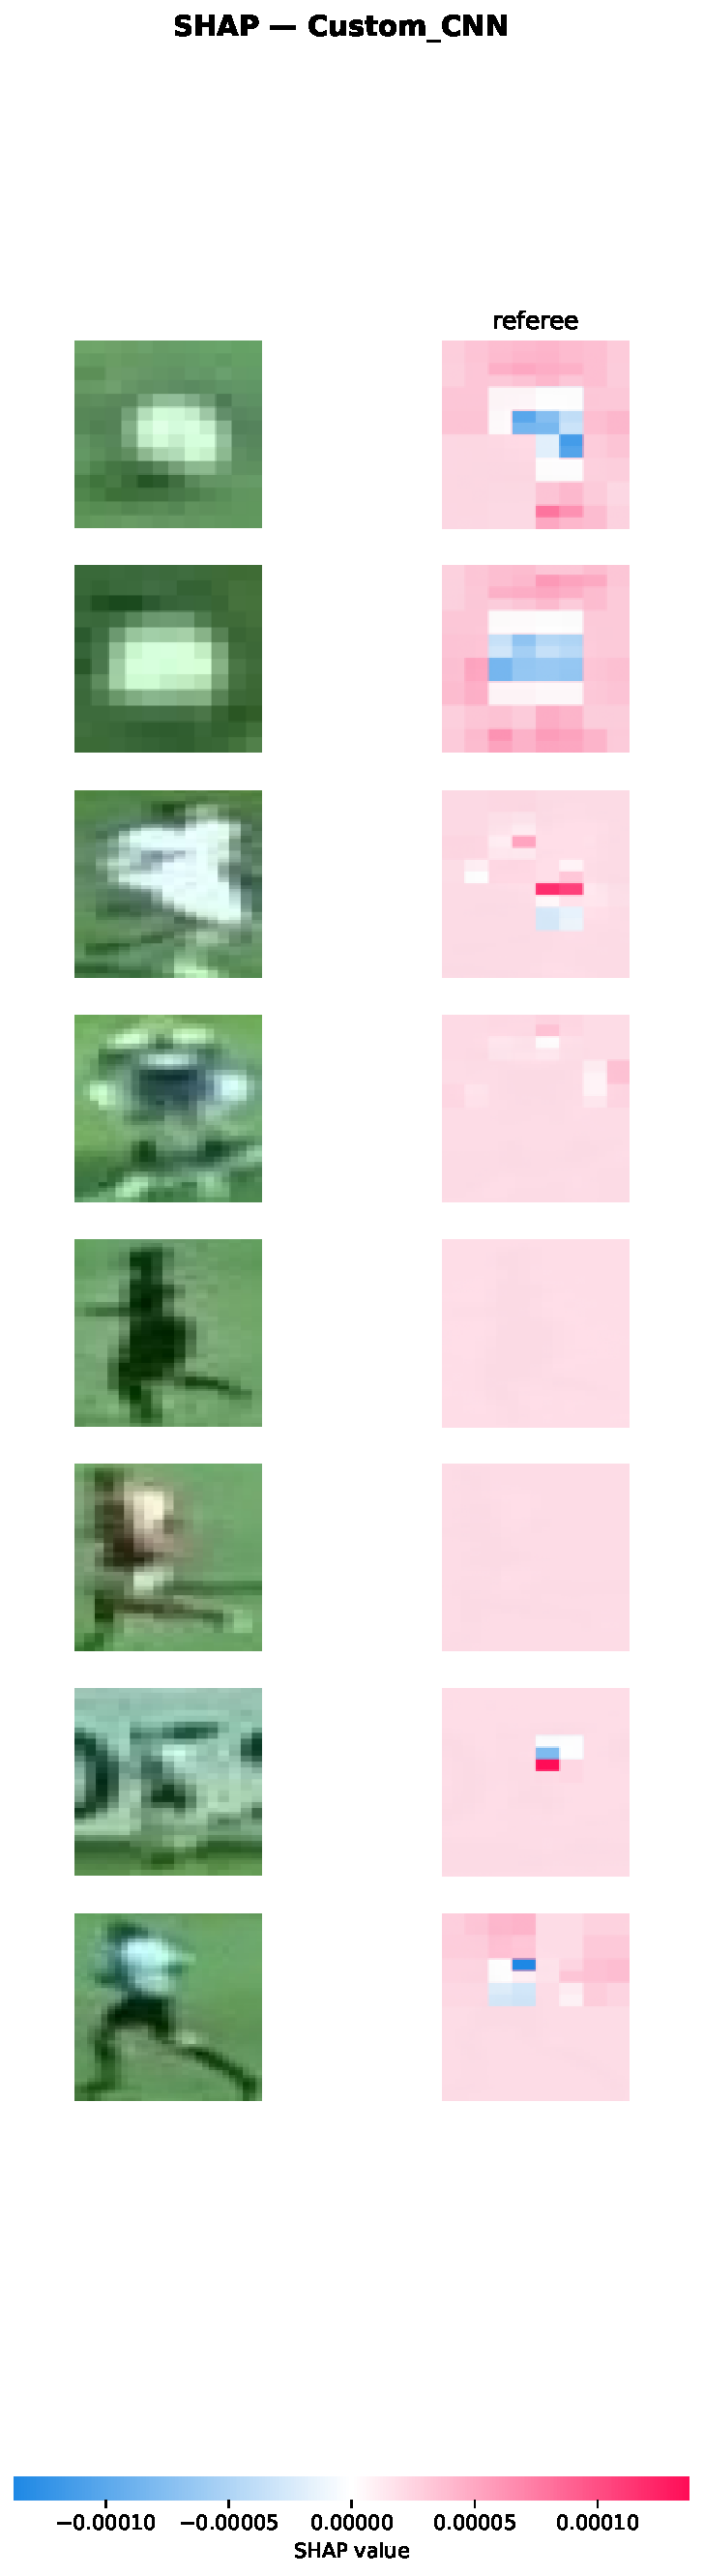
\includegraphics[width=0.95\columnwidth]{shap_Custom_CNN.pdf}
\caption{SHAP attribution maps for the custom CNN on two test crops per class. Red regions support and blue regions oppose the predicted class; supporting evidence falls mainly on the object itself, in agreement with the Grad-CAM analysis.}
\label{fig:shap_cnn}
\end{figure}

\begin{figure}[!ht]
\centering
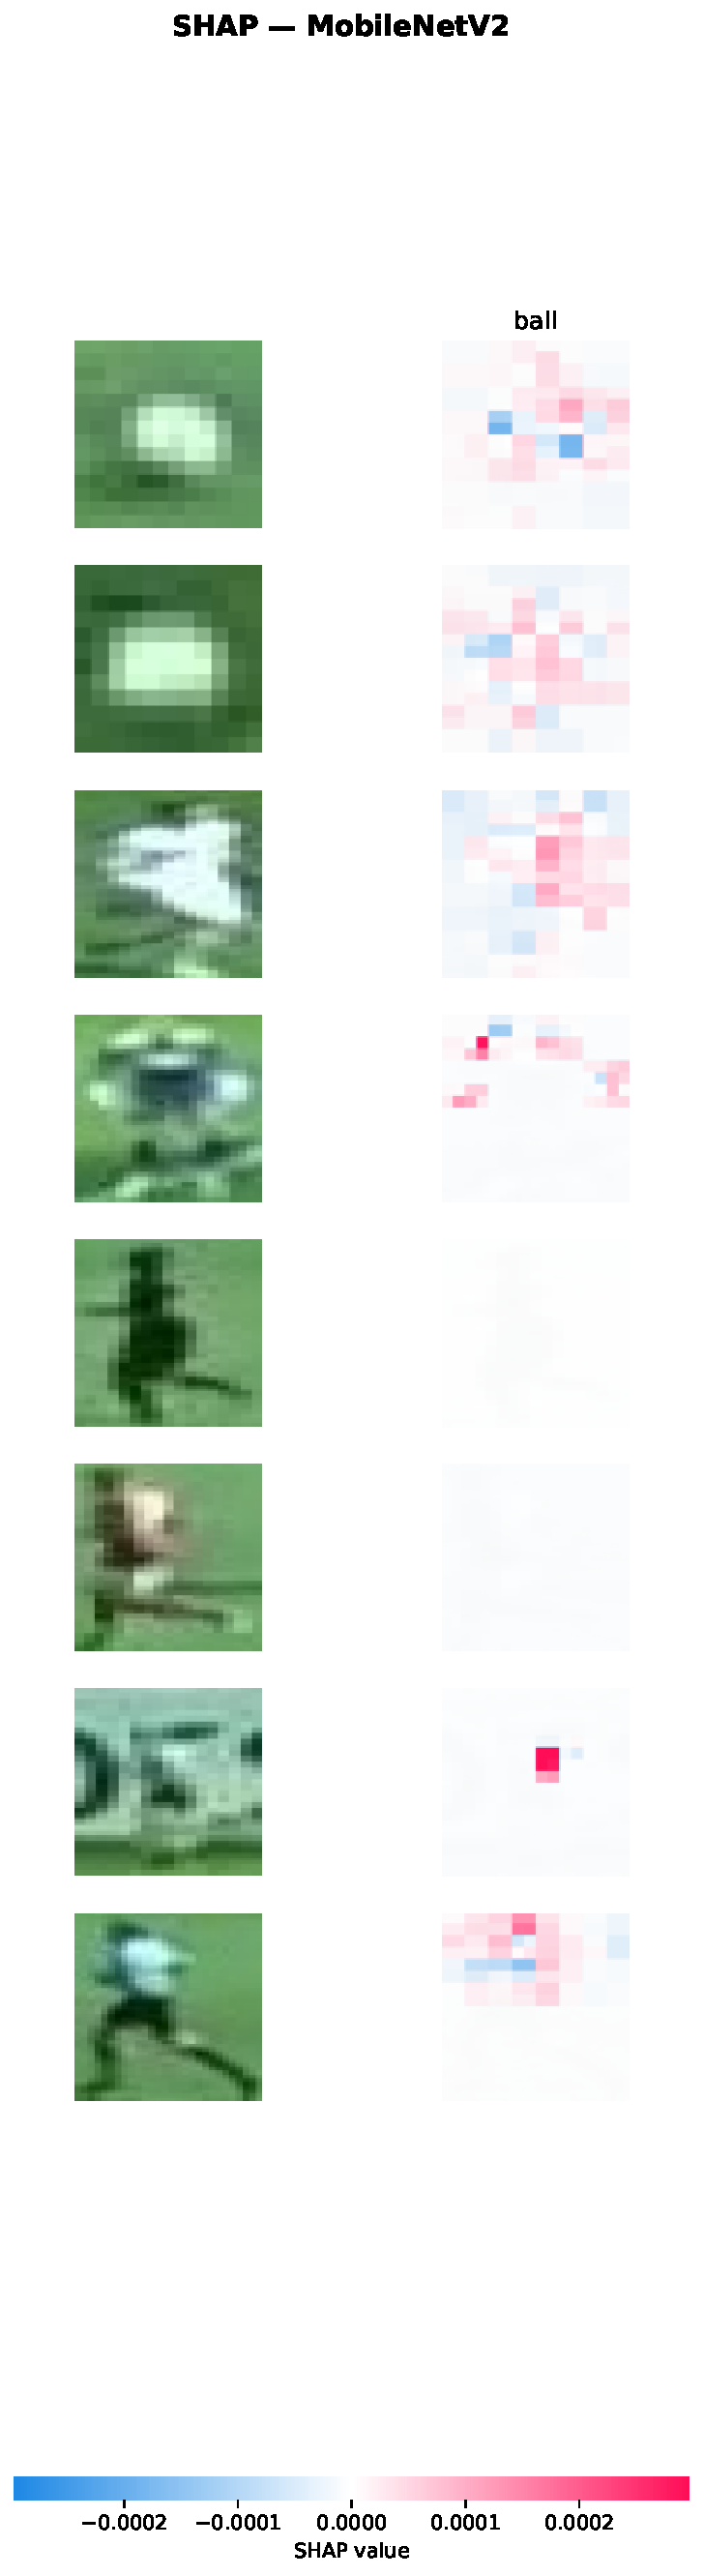
\includegraphics[width=0.95\columnwidth]{shap_MobileNetV2.pdf}
\caption{SHAP attribution maps for MobileNetV2. Supporting regions concentrate on the object of interest for the ball and player classes, consistent with the model's stronger performance on those roles.}
\label{fig:shap_mobile}
\end{figure}

\begin{figure}[!ht]
\centering
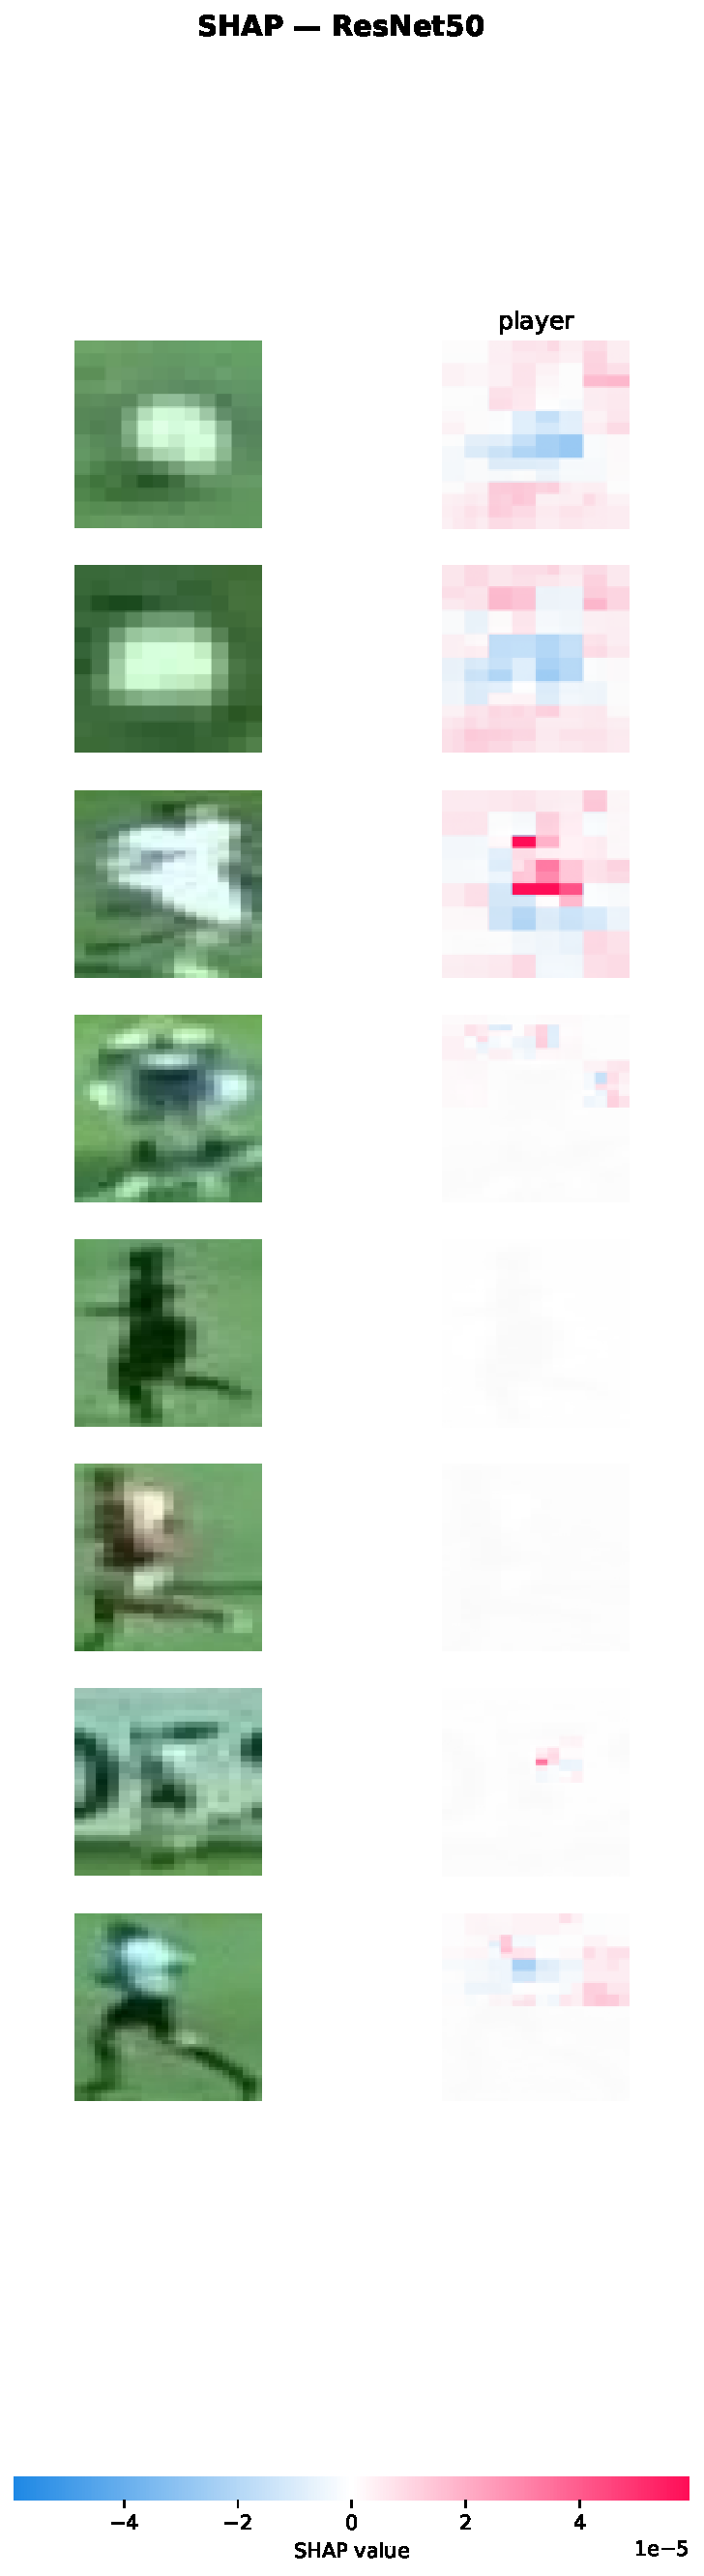
\includegraphics[width=0.95\columnwidth]{shap_ResNet50.pdf}
\caption{SHAP attribution maps for ResNet50. The attributions are weak and scattered across the background rather than the object, reflecting that the prediction is effectively independent of image content because the model always outputs the player class.}
\label{fig:shap_resnet}
\end{figure}

\subsection{Robustness Results}
Figure~\ref{fig:robustness} reports test accuracy under five corruptions at five severity levels.
The custom CNN degrades gracefully under mild blur and occlusion but drops sharply under reduced brightness, falling from 77.9\% on clean images to roughly 9\% at the most severe darkening, and it is also strongly affected by additive noise.
MobileNetV2 is comparatively resilient to blur and JPEG compression, in some cases even improving slightly at moderate severities because smoothing removes high-frequency clutter, yet it collapses under heavy noise, darkening, and large occlusion.
ResNet50 produces an exactly constant accuracy of 84.0\% and macro F1-score of 0.23 across every corruption and every severity, including the most extreme ones.
This perfect invariance is not a sign of robustness but a direct consequence of the model always predicting the player class regardless of the input, which the corruption analysis exposes unambiguously.
The robustness results therefore reinforce the explainability findings and inform RQ5 by showing that the custom CNN, while not the most accurate under all corruptions, is the only model whose predictions actually respond to the image.

\begin{figure*}[!ht]
\centering
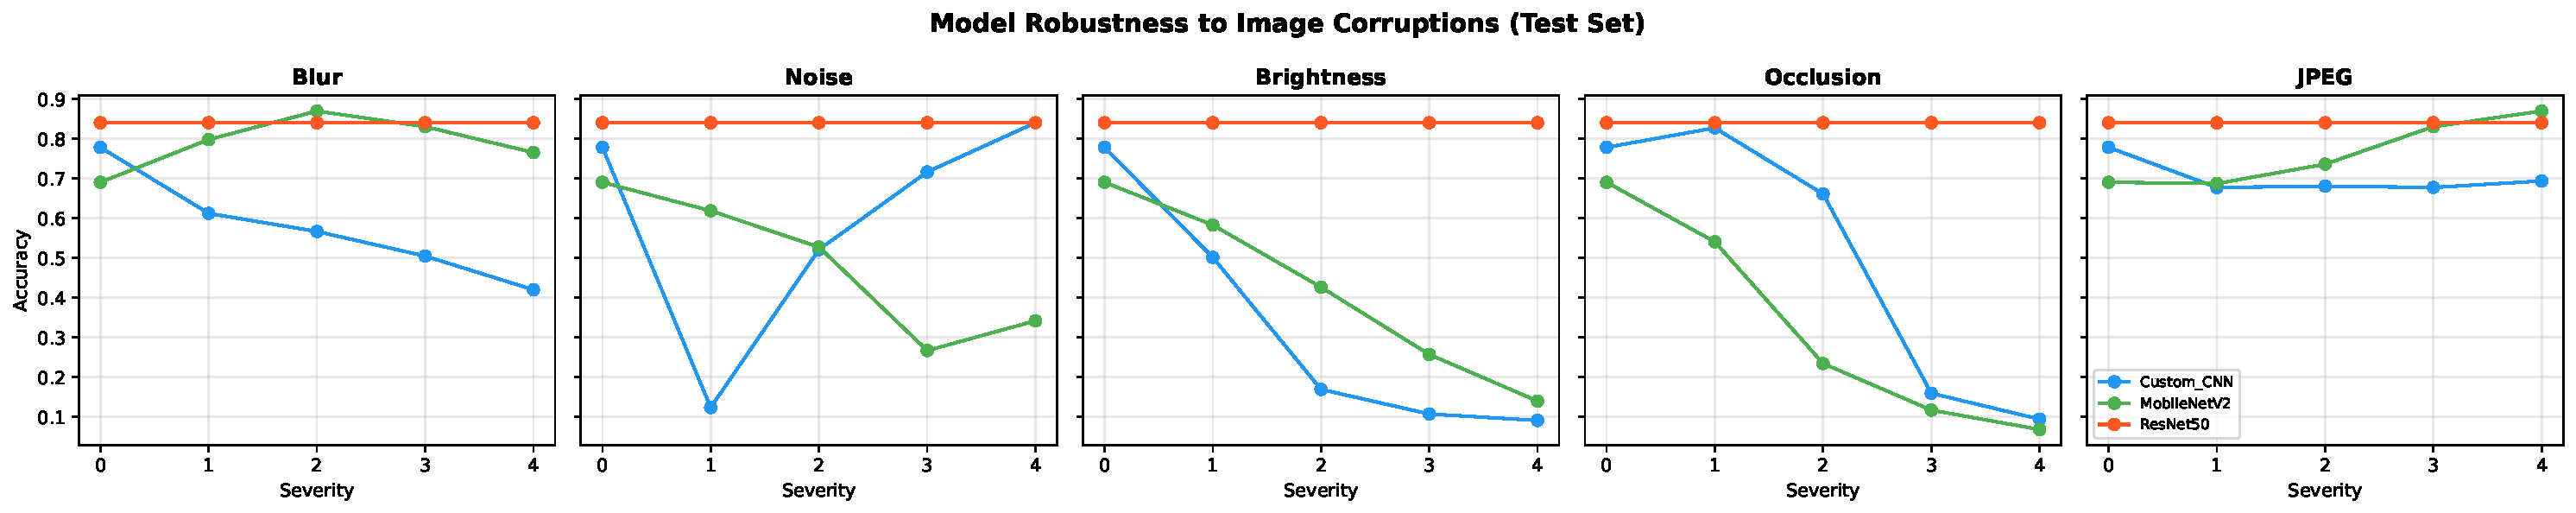
\includegraphics[width=17.8cm]{robustness_accuracy.pdf}
\caption{Test accuracy under five broadcast-like corruptions (blur, additive noise, reduced brightness, central occlusion, and JPEG compression) at five severity levels, with severity zero denoting the clean image. The custom CNN and MobileNetV2 respond to the corruptions as expected, whereas ResNet50 yields a perfectly flat curve because it predicts the majority class for every input, demonstrating that its apparent invariance is a degenerate artefact rather than genuine robustness.}
\label{fig:robustness}
\end{figure*}

\subsection{Efficiency and Deployment Results}
The efficiency columns of Table~\ref{tab:results} show a more than fifty-fold difference in size between the custom CNN and ResNet50, at 0.46 million versus 24.8 million parameters and 5.4\,MB versus 147\,MB on disk.
MobileNetV2 sits between them at 3.05 million parameters and 30\,MB.
The accuracy-efficiency trade-off strongly favours the custom CNN, which delivers the best macro F1-score while being by far the smallest and cheapest to store and run.
This result is central to RQ5, because the most deployable model on modest hardware is also the most balanced, removing any tension between efficiency and reliability for this task.
Figure~\ref{fig:inference} illustrates a qualitative deployment scenario in which a model is applied to a full match frame with annotated bounding boxes.

\begin{figure*}[!ht]
\centering
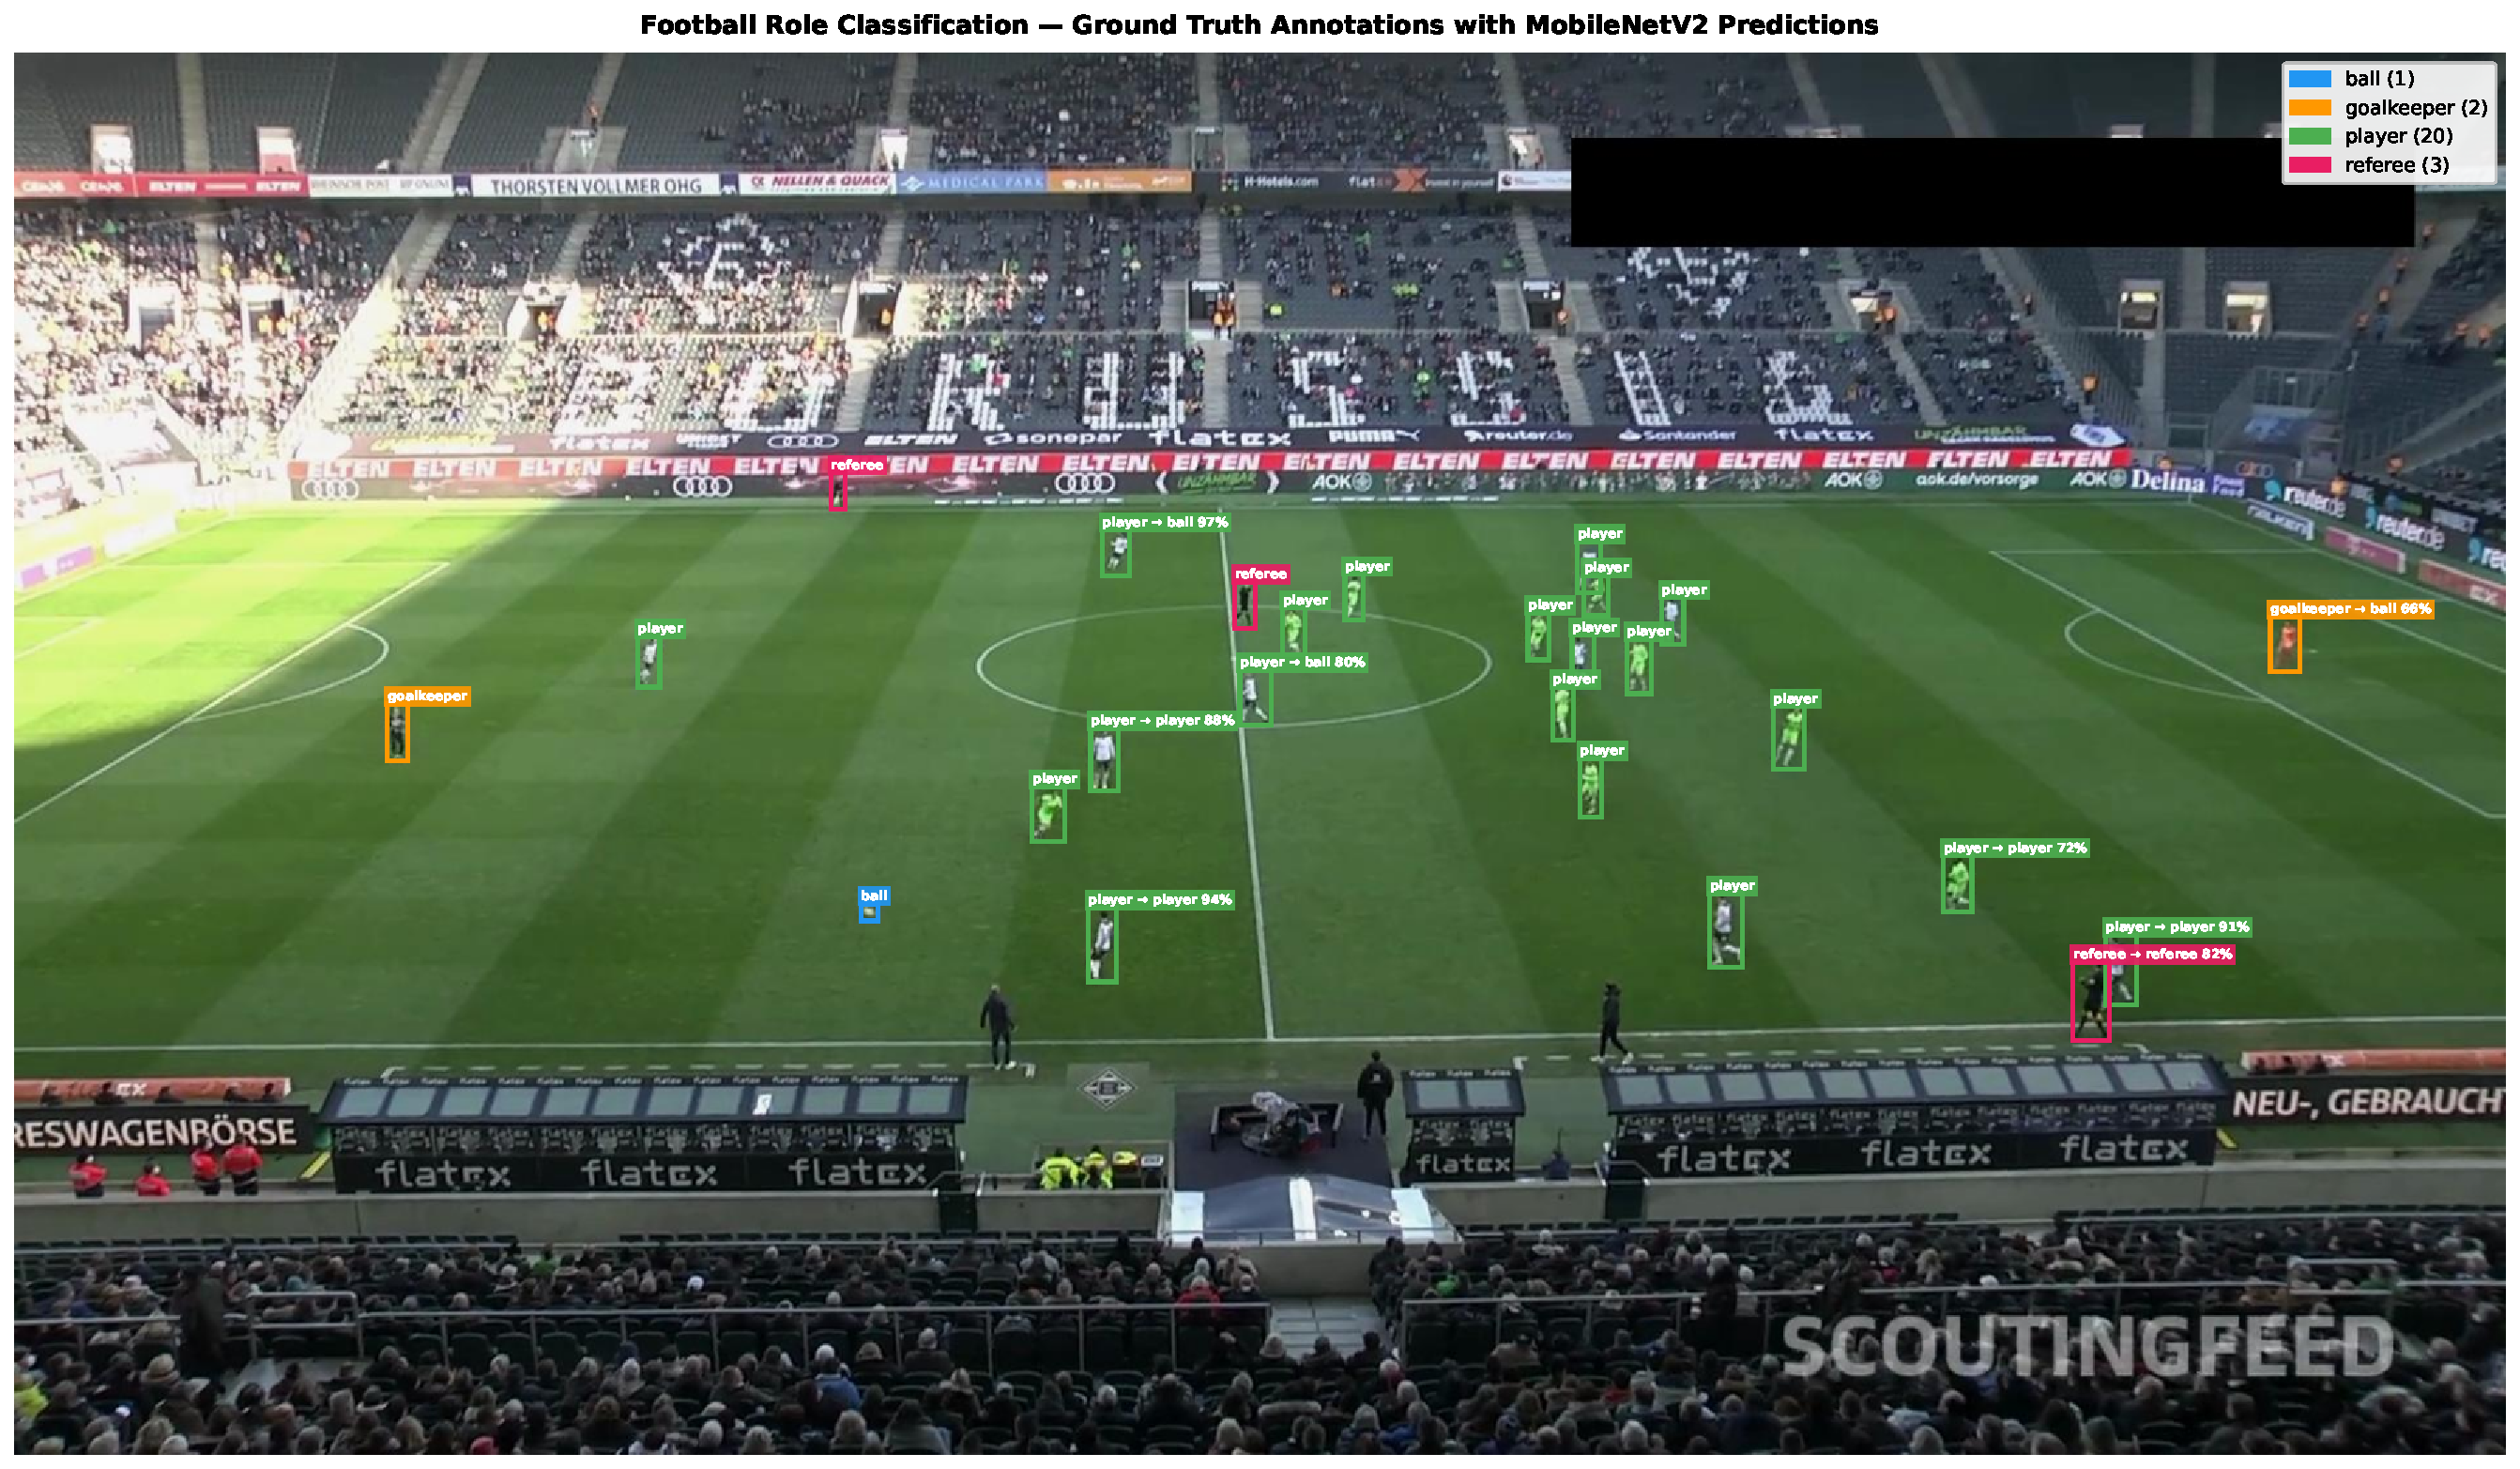
\includegraphics[width=15cm]{inference_demo.pdf}
\caption{Qualitative inference on a real match frame, with ground-truth bounding boxes coloured by class (ball, goalkeeper, player, referee). For objects large enough to classify reliably the predicted role and confidence are shown next to the true label, illustrating both correct predictions and the characteristic confusion between goalkeepers, referees, and distant players.}
\label{fig:inference}
\end{figure*}

\subsection{Comparison with Published Studies}
A direct numerical comparison with published football studies is limited because most report detection mean average precision on different datasets and splits rather than four-class crop-classification F1-scores~\cite{giancola2018soccernet,deliege2021soccernetv2,somers2024multitask}.
Detection-oriented works consistently report that the ball is the hardest object owing to its small size, whereas in the present crop-classification setting the ball is among the easiest classes once it is correctly localised, because its round shape is highly distinctive.
The goalkeeper difficulty observed here mirrors the role-confusion challenges reported in role-aware sports studies, where appearance similarity between roles is a recurring obstacle~\cite{somers2024multitask}.
The observation that a lightweight model can match or exceed a much deeper one on small data is consistent with comparative transfer-learning studies in other domains~\cite{martins2025mobilenet}.
These comparisons are qualitative by necessity, and the differences in dataset, split, and evaluation protocol are stated explicitly rather than glossed over.

\subsection{Summary of Research-Question Findings}
Table~\ref{tab:rqsummary} summarises the evidence and principal result for each research question.

\begin{table}[!ht]
\centering
\caption{Summary of research-question findings, listing the evidence used and the principal result for each question; all five questions are answered by the reported experiments.}
\label{tab:rqsummary}
\begin{tabular}{p{0.5cm} p{3.2cm} p{3.4cm} c}
\toprule
\textbf{RQ} & \textbf{Evidence} & \textbf{Principal result} & \textbf{Answered} \\
\midrule
RQ1 & Test accuracy and macro F1 (Table~\ref{tab:results}) & Roles are classifiable, but accuracy alone is misleading & \cmark \\
RQ2 & Three-model comparison (Tables~\ref{tab:results},~\ref{tab:perclass}) & The custom CNN is best by macro F1; ResNet50 collapses & \cmark \\
RQ3 & Balancing, per-class metrics, confusion matrices & Balancing helps minority roles; goalkeeper is hardest & \cmark \\
RQ4 & Grad-CAM and SHAP (Figs.~\ref{fig:gradcam_cnn}--\ref{fig:shap_resnet}) & CNN/MobileNetV2 attend to objects; ResNet50 does not & \cmark \\
RQ5 & Robustness and efficiency (Fig.~\ref{fig:robustness}, Table~\ref{tab:results}) & The smallest model is the most balanced and deployable & \cmark \\
\bottomrule
\end{tabular}
\end{table}

\section{Discussion}
\label{sec:discussion}

\subsection{Interpretation of Dataset and Preprocessing Findings}
The dataset and preprocessing results show that imbalance, not raw image difficulty, is the defining characteristic of this problem, which directly informs RQ1.
Label-preserving augmentation visibly stabilised training of the custom CNN, whose validation curve tracked its training curve without a large generalisation gap.
Training-only balancing was decisive for the minority roles, because it gave the discriminative models enough ball and goalkeeper examples to learn from while leaving the evaluation distribution realistic.
The decision to balance only the training split, and to preserve the natural distribution in validation and test, means the reported metrics reflect genuine deployment conditions rather than an artificially easy balanced test.
Preprocessing preserved the kit-colour cues that separate the roles, which matters because aggressive colour augmentation would likely have harmed the already difficult goalkeeper and referee classes.
The quality issues identified earlier, especially tiny ball crops and goalkeeper-player similarity, reappear consistently in the error analysis, confirming that they are intrinsic to the data.
These observations are consistent with imbalanced-learning and augmentation surveys that warn against evaluating on artificially balanced test sets and against label-altering transformations~\cite{ghosh2024imbalance,lewy2023augmentation}.

\subsection{Comparative Performance of CNN Models}
The comparison answers RQ2 in a way that contradicts the naive reading of accuracy.
ResNet50 achieved the highest accuracy precisely because it learned the trivial solution of always predicting the majority class, which is rewarded by accuracy but punished by macro F1-score.
This is a textbook manifestation of the class-imbalance failure mode, in which a high-capacity model on insufficient and skewed data converges to the majority prior rather than to a discriminative solution~\cite{ghosh2024imbalance}.
The custom CNN performed best by macro F1-score because its limited capacity, combined with balancing and class weighting, made the lazy majority-class solution less attractive than actually separating the roles.
MobileNetV2 sat between the two, benefiting from pre-trained features but partially affected by the same imbalance pressure that overwhelmed ResNet50.
Fine-tuning helped MobileNetV2 more than ResNet50, which is consistent with the observation that lighter backbones adapt more gracefully to small datasets~\cite{martins2025mobilenet,sandler2018mobilenetv2}.
The practically meaningful conclusion is that the highest accuracy does not identify the best model, and that model selection on this task must be driven by macro F1-score and per-class behaviour.

\subsection{Class-Level Reliability and Error Patterns}
The class-level analysis answers RQ3 and explains where and why the models fail.
The ball was the easiest class for the two functioning models because its round shape and high contrast are highly distinctive once cropped, whereas the goalkeeper was the hardest because it is visually almost identical to an outfield player and is severely underrepresented.
Referees were intermediate, recognisable by their neutral kit but confusable with goalkeepers at distance.
The dominant error for the custom CNN and MobileNetV2 is therefore confusion among the three human roles, while ResNet50's errors are categorical, since it never predicts anything but player.
In a deployment context the consequences differ by error type, as missing the ball would break ball-tracking analytics, whereas confusing a goalkeeper with a player would distort positional statistics.
The combination of small class size and high visual similarity is the root cause, and it is the same difficulty reported in role-aware sports studies~\cite{somers2024multitask}.
These error patterns also indicate that simply collecting more goalkeeper crops would likely yield the largest single improvement.

\subsection{Interpretation of Grad-CAM and SHAP}
The explainability analysis answers RQ4 and is arguably the most important result of the study.
For the custom CNN and MobileNetV2, both Grad-CAM and SHAP show that predictions are driven by the object of interest, which increases confidence that these models reason from meaningful evidence.
For ResNet50, neither method shows consistent object-focused evidence, which reveals that its high accuracy is produced without using class-specific image content at all.
The agreement between two methodologically different explanation techniques makes this conclusion robust, because it cannot be dismissed as an artefact of a single method's known instabilities~\cite{nazir2023survey}.
This case is a concrete demonstration of why attractive aggregate metrics must never be treated as proof of correct reasoning, and why explainability belongs in the evaluation rather than as a decorative addition.
At the same time the explanations must be read with appropriate caution, since Grad-CAM is spatially coarse and SHAP depends on the masking baseline, so they are used here as corroborating rather than definitive evidence.
For an application that could eventually touch officiating or commercial analytics, this kind of verification is essential before any model is trusted.

\subsection{Efficiency and Practical Deployment}
The efficiency analysis answers RQ5 and is unusually clear-cut for this task.
There is normally a trade-off between accuracy and efficiency, but here the smallest model is also the most reliable by macro F1-score, so no such compromise is required.
The custom CNN occupies 5.4\,MB and has fewer than half a million parameters, which makes it suitable for deployment on commodity hardware, edge devices, or in-browser inference, whereas ResNet50 at 147\,MB offers no reliability benefit to justify its cost.
MobileNetV2 remains a reasonable middle option when pre-trained features are desired, and its relative robustness to blur and compression could be valuable for low-quality broadcast feeds.
Any deployment would still require human oversight given the goalkeeper confusion, and image-acquisition quality, particularly resolution of distant objects, would materially affect real-world performance.
The operational risk of the degenerate ResNet50 behaviour is especially instructive, because such a model could pass a naive accuracy-based acceptance test and then fail silently in production.

\subsection{Comparison with Existing Literature}
The results support the broad finding in the imbalanced-learning literature that aggregate accuracy is an unsafe selection criterion, and they extend it to the football role-classification setting~\cite{ghosh2024imbalance}.
They also support comparative transfer-learning studies reporting that lightweight networks can match or exceed deeper ones on small data~\cite{martins2025mobilenet}.
The workflow here differs from typical sports-vision pipelines by isolating role classification as a standalone, explainable, and robustness-tested task rather than embedding it in a detector or tracker~\cite{giancola2018soccernet,somers2024multitask}.
Direct numerical comparison is difficult because datasets, splits, and metrics differ, and this limitation is stated rather than hidden.
The methodological contribution is therefore the integrated evaluation protocol, combining leakage-free splitting, dual explainability, and corruption robustness, rather than a claim of state-of-the-art accuracy.
No superiority claim is made over works using different protocols, in line with good comparative practice.

\subsection{Practical and Scientific Contributions}

\textbf{Scientific Contributions.}
The study provides a systematic, controlled comparison of a custom CNN against two transfer-learning backbones under identical conditions, an explainability-based reliability analysis that exposes a majority-class shortcut, a corruption-robustness analysis that independently confirms the shortcut, a class-level error analysis, and a fully reproducible methodology.
Together these show that macro F1-score, per-class metrics, and explanations are jointly necessary to evaluate models on imbalanced image tasks.

\textbf{Practical Contributions.}
For practitioners the study delivers a compact, deployable model that is reliable across all four roles, a warning that high-accuracy models may be silently degenerate, and a low-cost recipe suitable for resource-constrained clubs and analysts.
The pipeline can serve as a screening or pre-annotation tool that reduces manual labelling effort while keeping a human in the loop.

\subsection{Ethical, Social, and Safety Implications}
Although role classification is less sensitive than personal identification, broadcast imagery still involves real individuals, and any extension toward identification would raise privacy and consent concerns.
Unequal reliability across roles is itself a fairness issue, since decisions based on the underperforming goalkeeper class would be less dependable than those based on the player class.
If such a system were ever connected to officiating support, the risk of false reassurance from a degenerate but high-accuracy model would be serious, which is why human verification is mandatory for any high-stakes use.
The study therefore treats the framework strictly as decision support and recommends against autonomous use.

\subsection{Limitations}
Several limitations constrain the scope of the conclusions.
The dataset is small at 663 source images and is drawn from a single public source, which limits generalisation to other competitions, broadcasters, and camera setups.
The class imbalance is severe and the minority classes, especially the ball and goalkeeper, are represented by very few test crops, so their metrics are estimated from small samples.
Results come from a single training run per model with one split, so small differences are not statistically validated.
No external validation on an independent dataset was performed, and the hyperparameter search was limited by single-GPU resources.
The system classifies pre-cropped objects and does not perform detection, so it depends on an external localiser in practice.
These are genuine limitations of the present evidence rather than planned future activities.

\subsection{Future Research Directions}
The most valuable next step is to collect or combine larger and more balanced data, with particular emphasis on additional goalkeeper examples and on external validation across different leagues and broadcasters.
Repeated runs with confidence intervals and statistical significance tests would strengthen the reliability of the comparison.
Integrating the classifier with a detector such as a YOLO model would yield an end-to-end system that operates on full frames rather than pre-made crops~\cite{liang2025basketball}.
Further directions include evaluating additional efficient backbones such as EfficientNet, applying focal loss or other imbalance-aware objectives, adding uncertainty estimation so the model can abstain on ambiguous crops, and validating the explanations against domain-expert judgement.
Real-time and on-device deployment, together with data collected under genuine operating conditions, would test the framework's practical viability.

\section{Conclusion}
\label{sec:conclusion}
This study addressed the automatic classification of four on-pitch football roles, namely ball, goalkeeper, player, and referee, from broadcast image crops, using a comparative and explainable CNN-based framework.
A lightweight custom CNN was compared against fine-tuned MobileNetV2 and ResNet50 on a leakage-free, training-only-balanced version of a public dataset, and the models were interpreted with Grad-CAM and SHAP and stress-tested under five broadcast-like corruptions.
The principal finding is that the highest-accuracy model, ResNet50 at 84.0\%, is in fact the worst, because it collapses onto the majority class and reaches a macro F1-score of only 0.23, whereas the 0.46-million-parameter custom CNN delivers the best balanced performance at 77.9\% accuracy and a macro F1-score of 0.67.
The Grad-CAM and SHAP analyses independently confirmed that the custom CNN and MobileNetV2 attend to meaningful objects while ResNet50 does not, and the robustness analysis exposed ResNet50's pathological invariance to image corruption.
In practical terms the smallest and cheapest model is also the most reliable and deployable, which is a favourable outcome for resource-constrained users, provided that human oversight is retained because the goalkeeper class remains difficult.
The main limitation is the small, single-source, heavily imbalanced dataset evaluated on a single split, and the most promising future direction is to assemble a larger and better-balanced dataset, especially with more goalkeeper examples, and to validate the framework on independent broadcast footage.

\section*{Declarations}
The author used the generative AI tool ChatGPT (OpenAI, San Francisco, CA, USA) to improve the language and clarity of the manuscript.
The author reviewed and edited all content generated by the tool and takes full responsibility for the final version of the manuscript.

% DO NOT REMOVE THESE LINES AT ANY COST
\bibliographystyle{elsarticle-num}
\bibliography{Bibliography}

\end{document}
